%% V1.0
%% by Gabriel Garcia, gabrcg@gmail.com
%% This is a template for Udacity projects using IEEEtran.cls

%% Be Udacious!

\documentclass[10pt,journal,compsoc]{IEEEtran}

\usepackage[pdftex]{graphicx}    
\usepackage{cite}
\hyphenation{op-tical net-works semi-conduc-tor}


\begin{document}

\title{Map My World Robot}

\author{Hsin-Wen Chang}

\markboth{SLAM project, Robotics Nanodegree Program, Udacity}%
{}
\IEEEtitleabstractindextext{%

\begin{abstract}
This project leverage Real time Appearance Based mapping or RTAB-Map for Simultaneous localization and mapping which is the best solution to develop robots that can map environments in 3D. From RTAB-Map's speed and memory management, its custom developed tools for information analysis and, most importantly, the quality of the documentation. Being able to leverage RTAB-Map with our own robots will lead to a solid foundation for mapping and localization well. For this project we will be using the rtabmap ros package, which is a ROS wrapper (API) for interacting with rtabmap. Loop closure is detected using a bag of worlds approach which is commonly used in vision based mapping.
\end{abstract}

% Note that keywords are not normally used for peerreview papers.
\begin{IEEEkeywords}
Robot, IEEEtran, Udacity, \LaTeX, SLAM.
\end{IEEEkeywords}}

\maketitle
\IEEEdisplaynontitleabstractindextext
\IEEEpeerreviewmaketitle
\section{Introduction}
\label{sec:introduction}

\IEEEPARstart{S}{im}ultaneous localization and mapping (SLAM) is used for constructing and updating a map from unknown environment while keep tracking agent's location. In this project, SLAM was perform on two simulate 3D world where robot can mapping and localize them self by interface the robot with RTAB-Map addition of an RGB-D camera which allows robot estimate their trajectory and map feature pose through explore its environment and create high accuracy map of it's surround environment. The two environment should be mapped in 2D and 3D by using Gazebo and RViz.

\section{Background}
 When a mobile robot is mapping a large environment while traveling in cycles and correlating between different objects will face challenges and difficulties such as Unknown map, huge hypothesis space, size, noise, cycles and perceptual ambiguity. Mapping with know pose. The technologies combine localization and mapping process called Simultaneous localization and mapping (SLAM)[1].

\subsection{Occupancy Grid Mapping}
While listing the different challenges and difficulties in mapping, The words discrete and continuous:
\begin{itemize}
\item Discrete Data: You obtain this data by counting it. This data has finite values. Example: Number of robots in a room.

\item Continuous Data: You obtain this data by measuring it. This data has an infinite number of steps, which form a continuum. Occupancy Grid Mapping applied Posterior Probability implement a mapping algorithm and estimate the map given noisy measurements and assuming known poses.
\end {itemize}
\subsection{Grid-based FastSLAM}
The FastSLAM algorithm solves the Full SLAM problem by following:
%example for Bullet point list
\begin{itemize}
\item Estimating the Trajectory: FastSLAM estimates a posterior over the trajectory by applying particle filter approach which is an advantage to SLAM to solve the problem of mapping with known poses.
\item Estimating the Map: FastSLAM uses a low dimensional Extended Kalman Filter to solve independent features of the map which are modeled with local Gaussian. The custom approach of representing the posterior with particle filter and Gaussian is known by the Rao-Blackwellized particle filter approach.
\end {itemize}
\begin{figure}[thpb]
      \centering
      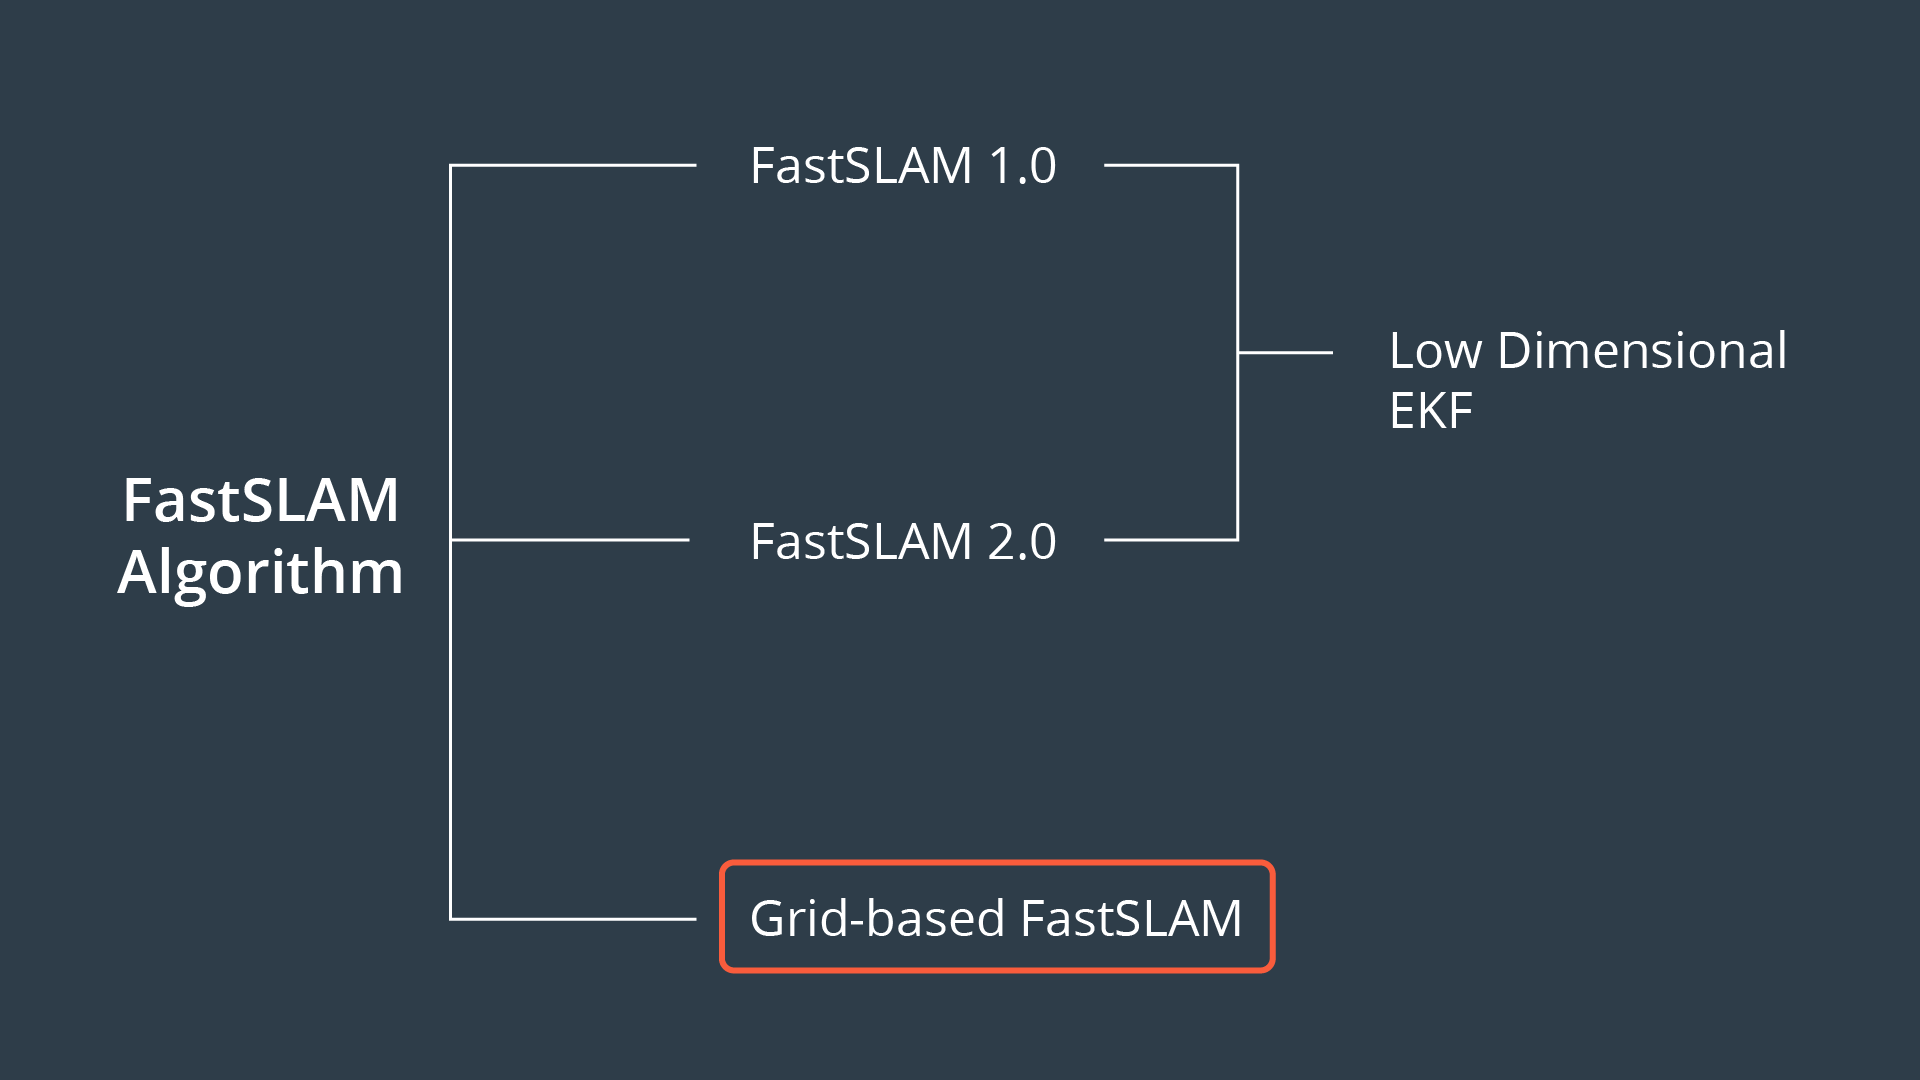
\includegraphics[width=\linewidth]{FastSLAM.png}
      \caption{FastSLAM.}
      \label{fig:robot1}
\end{figure}
\subsection{GraphSLAM}
GraphSLAM is a SLAM algorithm which solve the full SLAM problem and recovers the entire path and map instead of just recent pose and map.At the core of GraphSLAM is graph optimization - the process of minimizing the error present in all of the constraints in the graph by applying maximum likelihood estimation (MLE) to structure and solve the optimization problem for the graph.
In RTAB-Map, loop closure is detected using a bag of worlds approach which is commonly used in vision based mapping. When loop closure is disabled, you can see parts of the map output that are repeated, and the resulting map looks a lot more choppy. It is not an accurate representation of the environment. This is caused by the robot not using loop closure to compare new images and locations to ones that are previously viewed instead it registers them as new locations. When loop closure is enabled, the map is significantly smoother and is an accurate representation of the room and When a loop closure hypothesis is accepted, a new constraint is added to the map’s graph, then a graph optimizer minimizes the errors in the map. RTAB-Map supports 3 different graph optimizations: Tree-based network optimizer, or TORO, General Graph Optimization, or G2O and GTSAM (Smoothing and Mapping). All of these optimizations use node poses and link transformations as constraints. When a loop closure is detected, errors introduced by the odometry can be propagated to all links, correcting the map.
\begin{figure}[thpb]
      \centering
      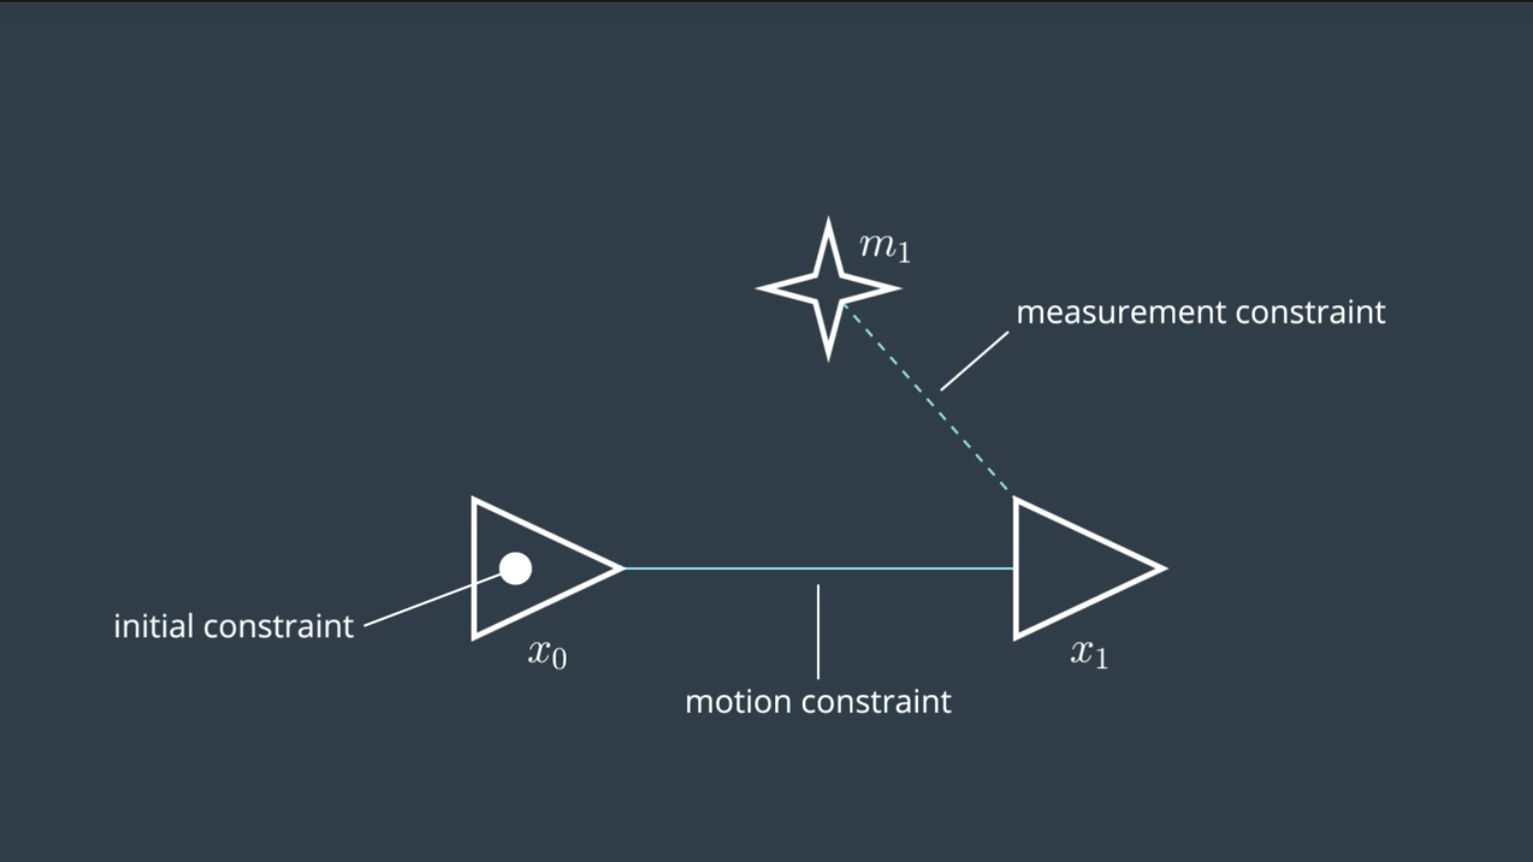
\includegraphics[width=\linewidth]{GraphSLAM.png}
      \caption{GraphSLAM.}
      \label{fig:robot1}
\end{figure}
\section{Scene and robot configuration}
\subsection{Robot Configuration}
Hsin bot was designed from previous project where am I. Most of the configuration of parameters in Hsin bot is base on Udacity bot except laser max beams to 20 in each scan to be used when updating the filter. Minimum allowed 50 number of particles. Maximum allowed 200 number of particles. Some adjustment were made by replace RGB-camera with RGB-D camera in order to measure depth for mapping with RTAB-MAP
\subsection{Kitchen and dining scene}
The Kitchen and dining scene was provided by Udacity as benchmark scene.
\begin{figure}[thpb]
      \centering
      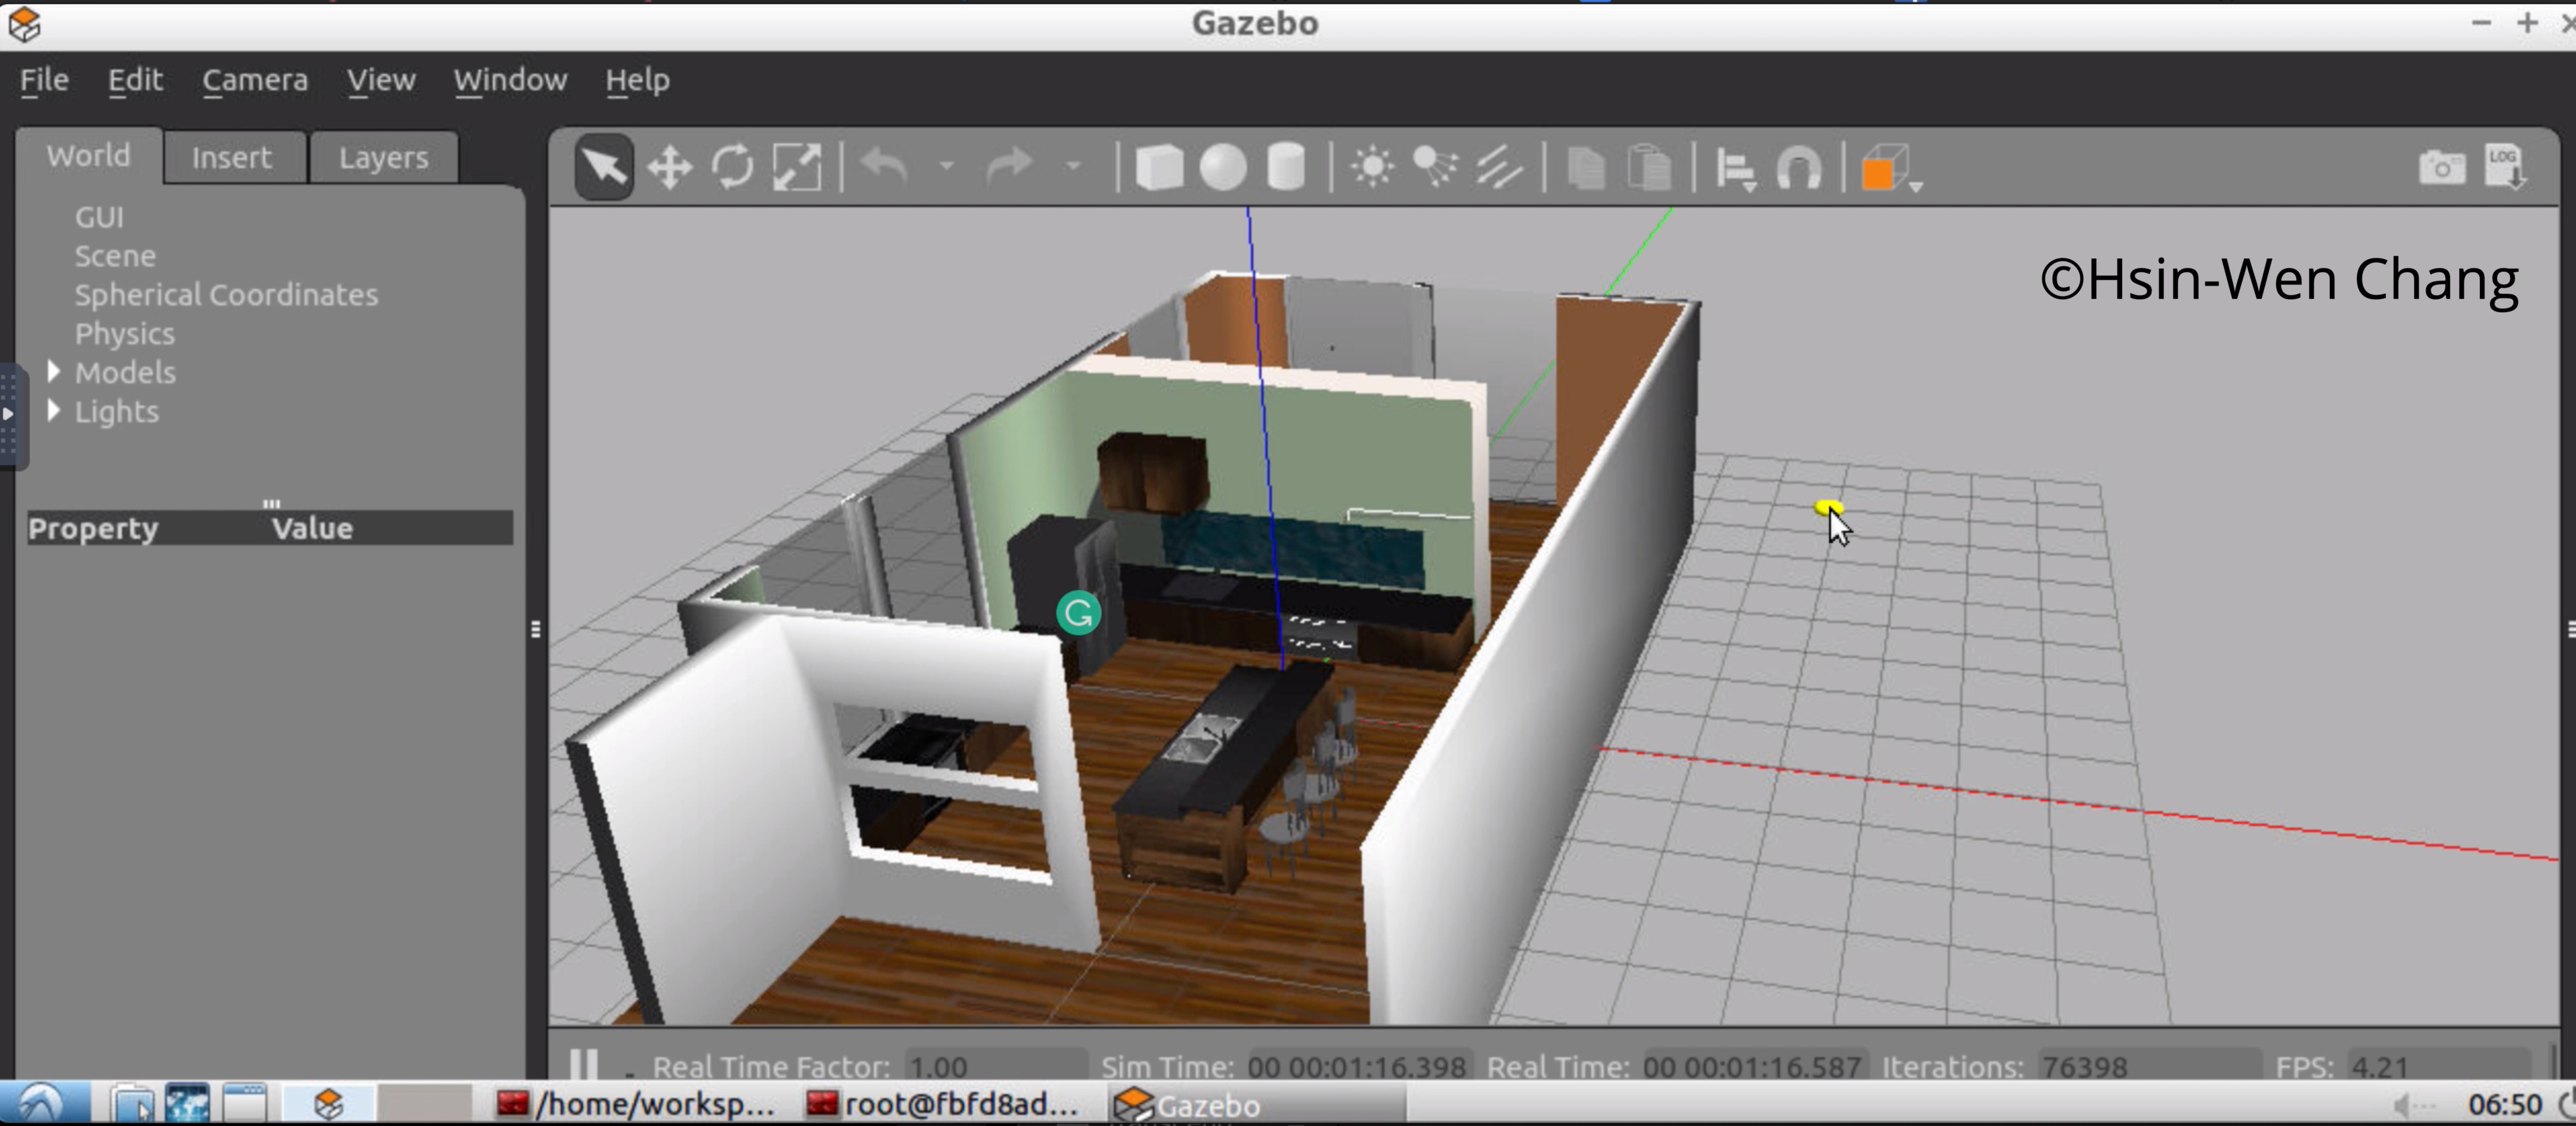
\includegraphics[width=\linewidth]{MapMyworld.png}
      \caption{Kitchen and dining scene A.}
      \label{fig:robot1}
\end{figure}
\begin{figure}[thpb]
      \centering
      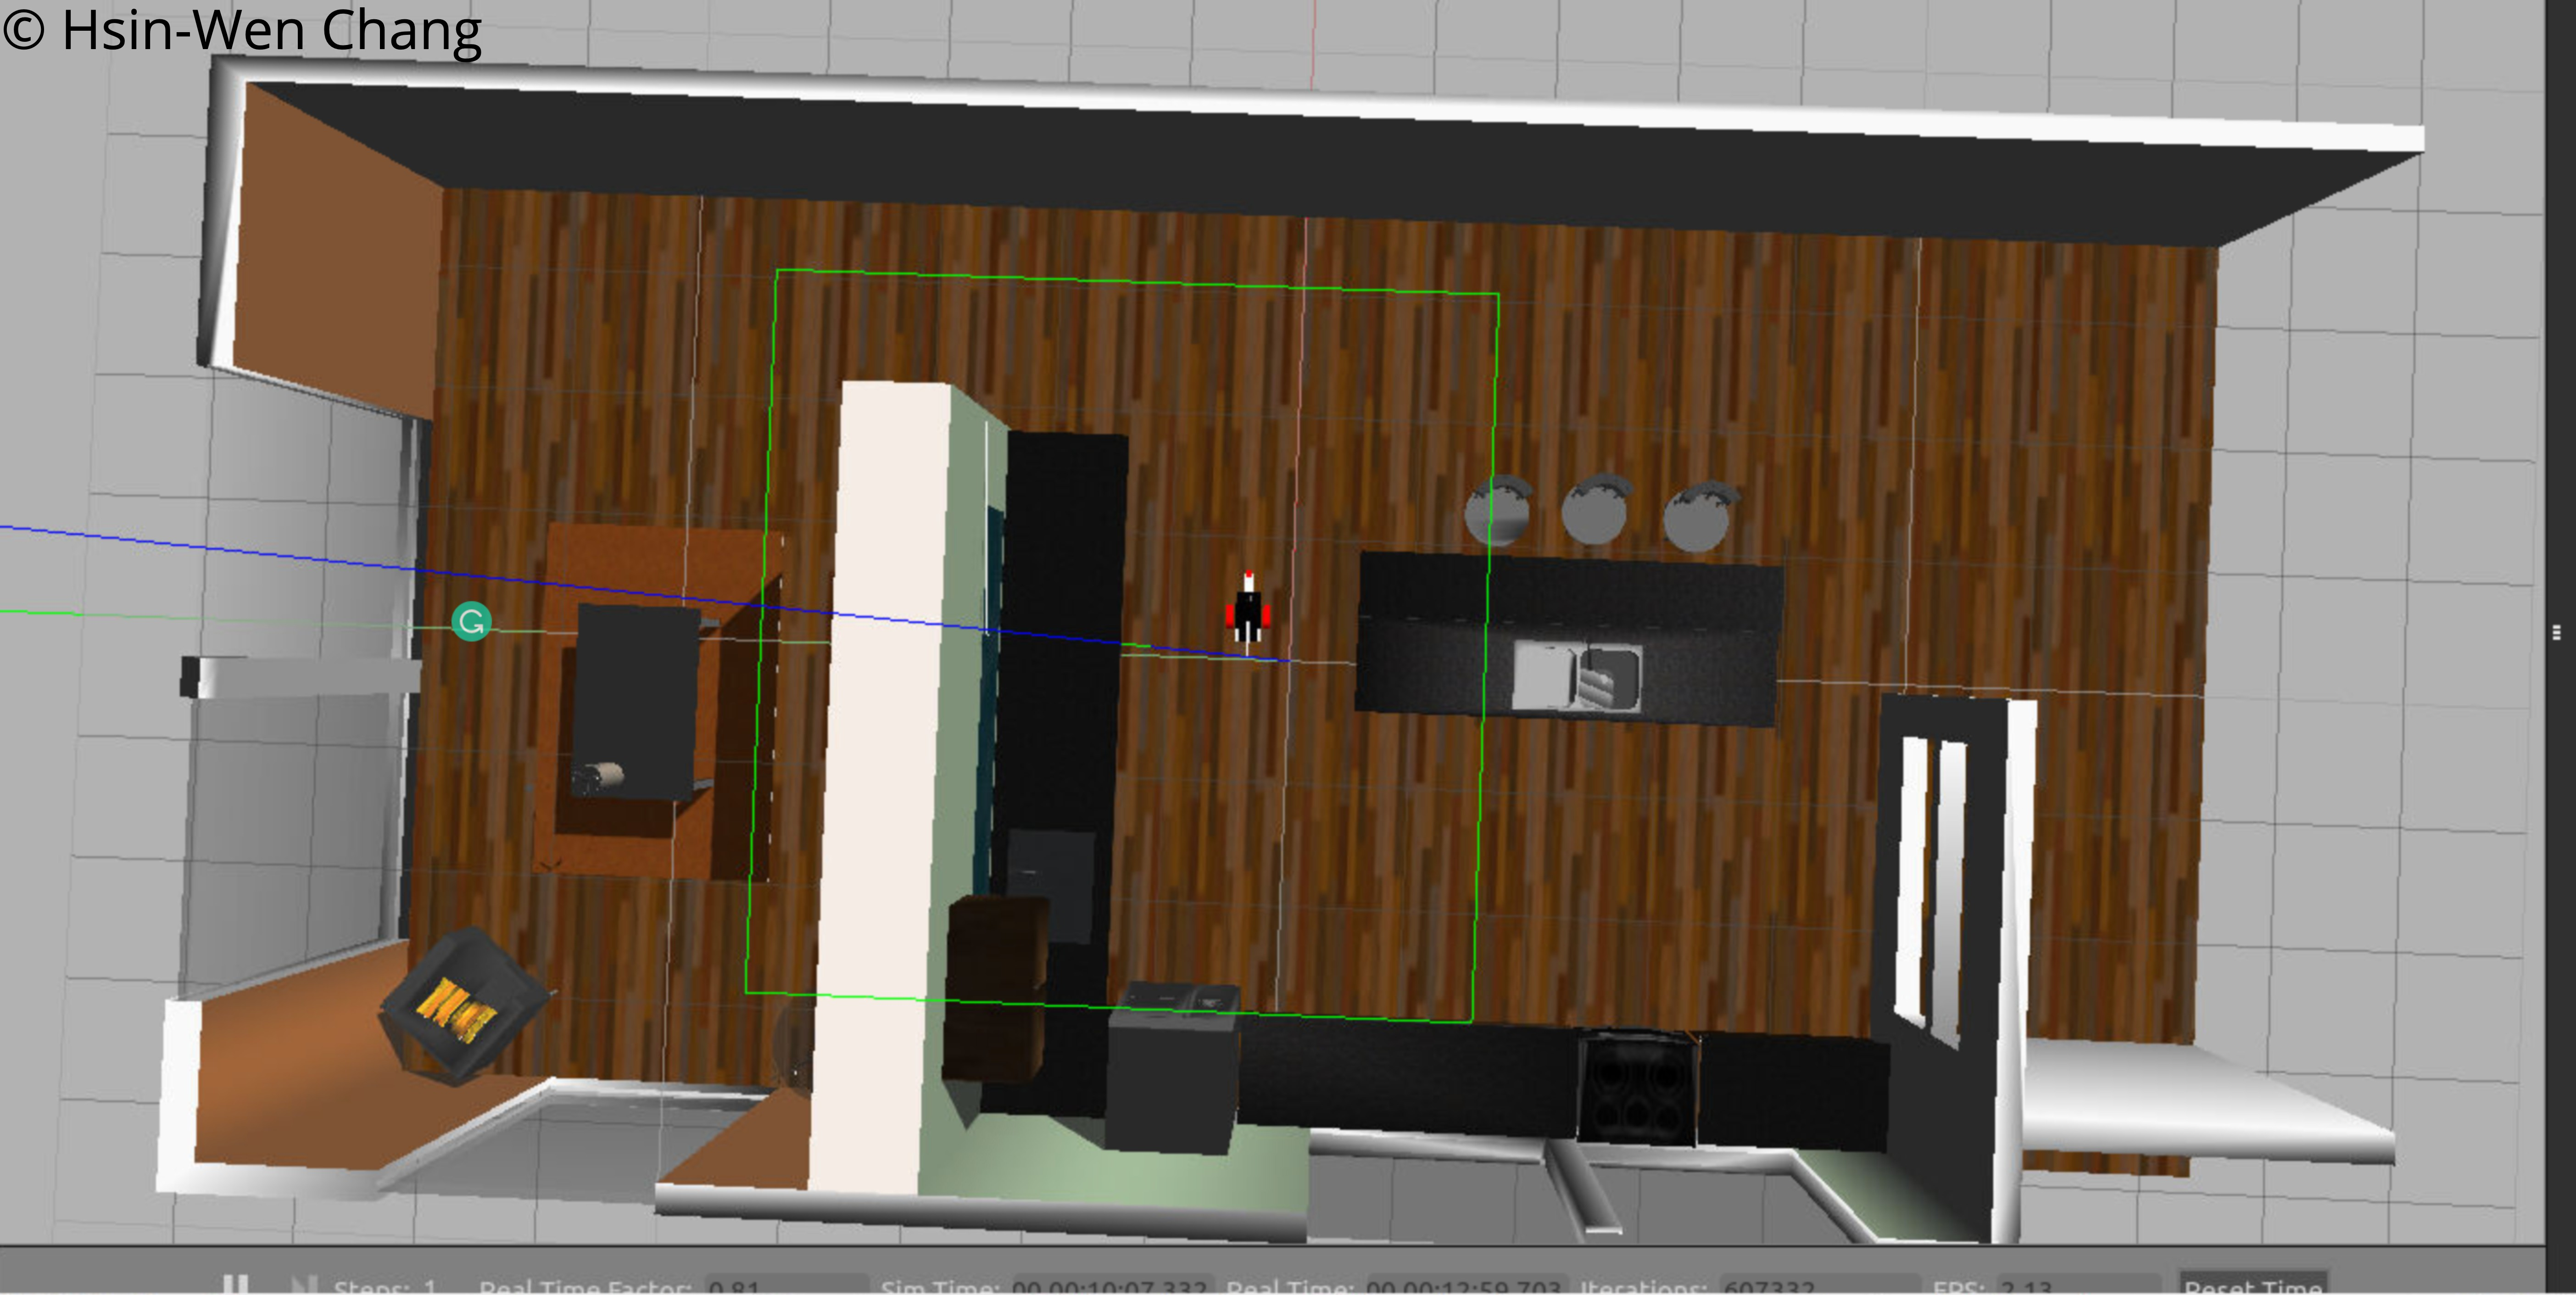
\includegraphics[width=\linewidth]{HsinBot.png}
      \caption{Kitchen and dining scene B.}
      \label{fig:robot1}
\end{figure}
\subsection{My World scene}
In here by applying scene willow garage which have many wall feature and alley for Hsin bot to capture during mapping.

\begin{figure}[thpb]
      \centering
      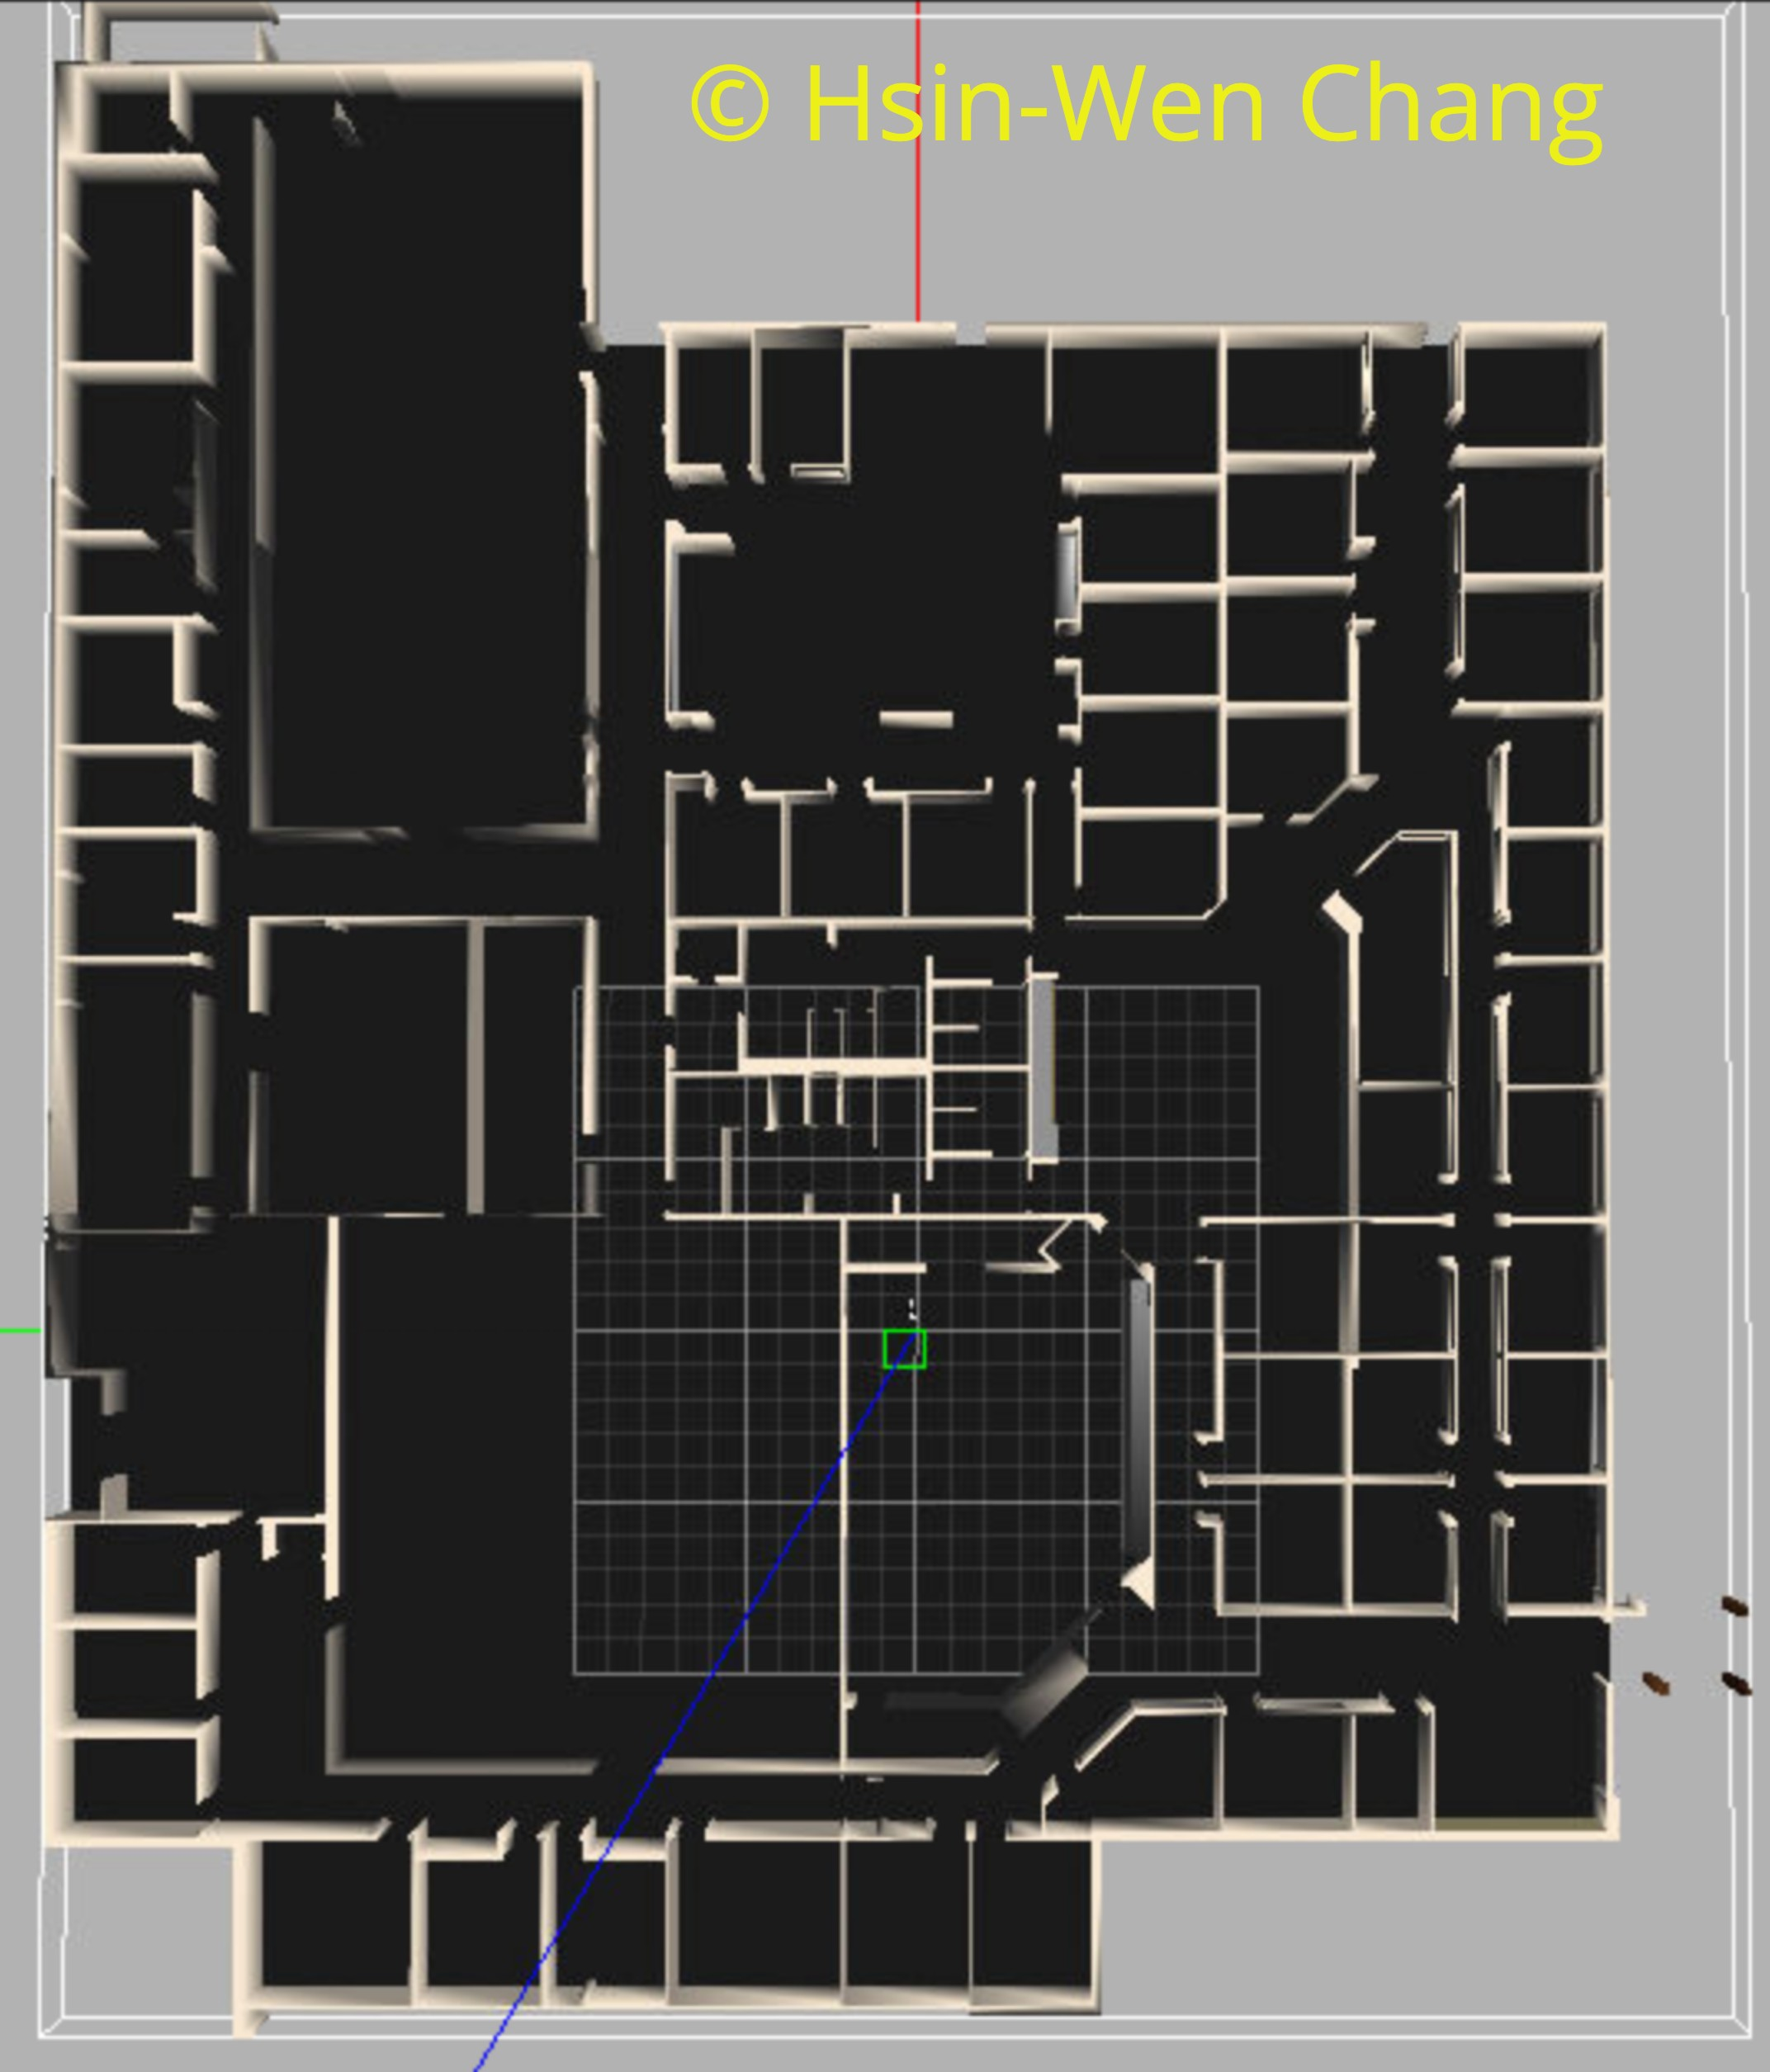
\includegraphics[width=\linewidth]{willowgarage.png}
      \caption{Willow Garage.}
      \label{fig:robot1}
\end{figure}
\begin{figure}[thpb]
      \centering
      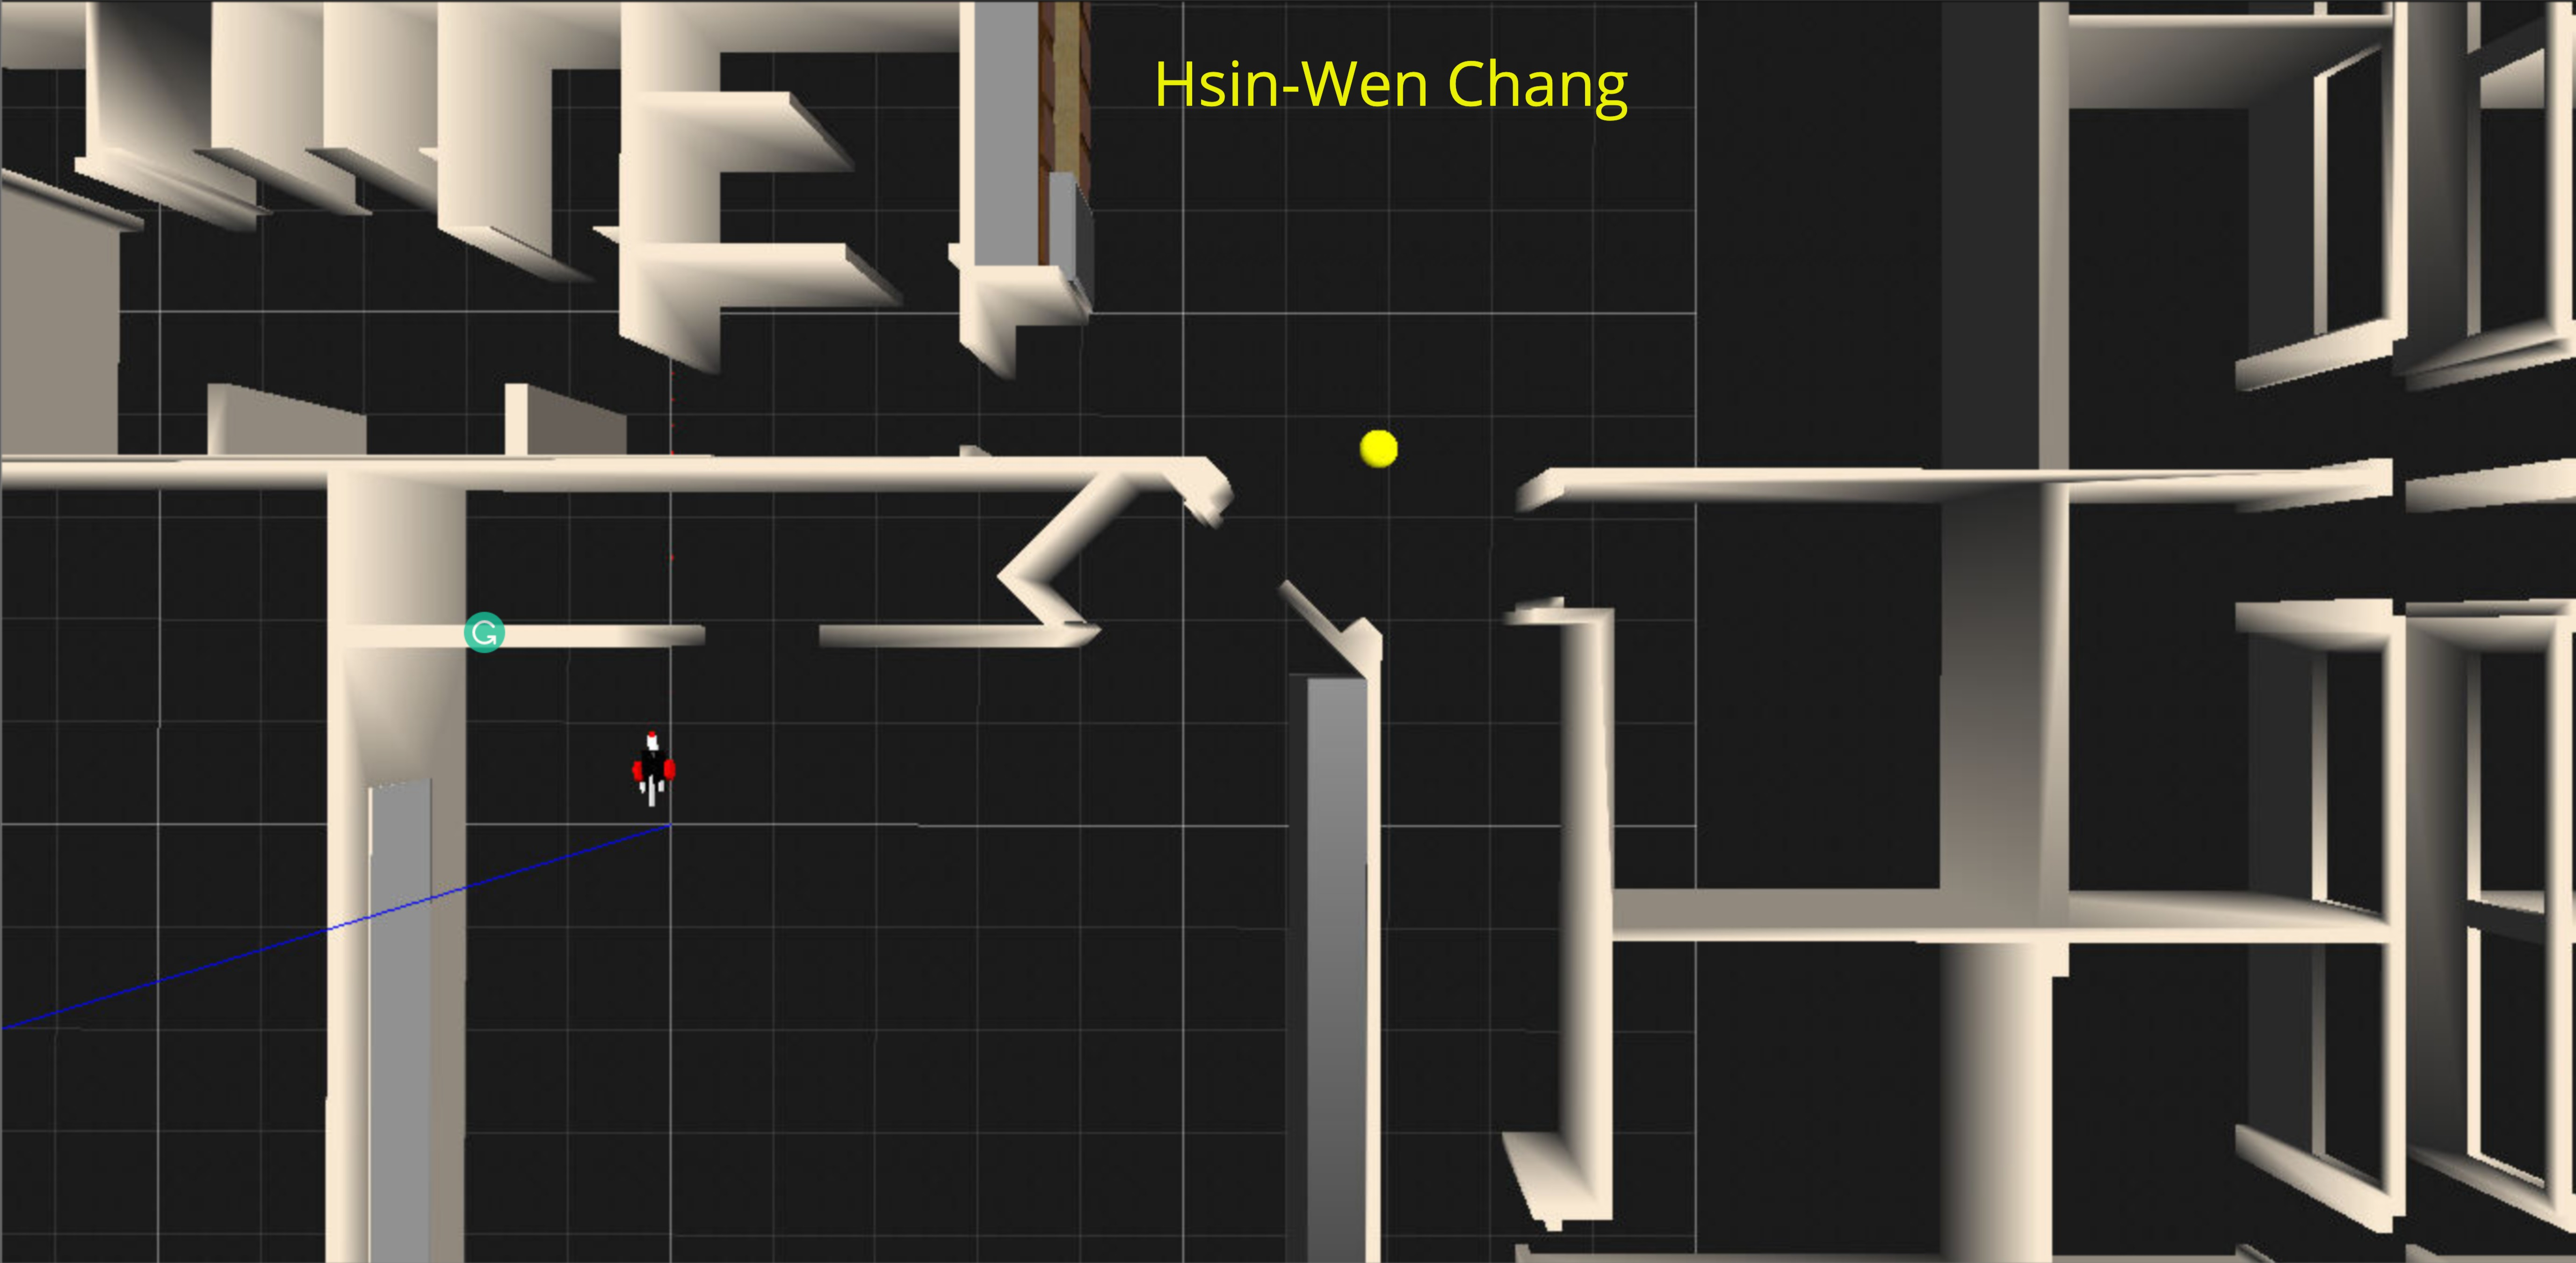
\includegraphics[width=\linewidth]{willowgarageHsinBot.png}
      \caption{HsinBot in willow garage.}
      \label{fig:robot1}
\end{figure}

\subsection{Robot configuration: Transformation frame}
Both of scenes are mapped by the designed robot which based on Udacity bot configuration and equipped with RGB-D camera which is the link attached to the RGB-D camera node in the .gazebo file and laser scanner. RTAB-MAP algorithm will augment the depth measurements of the RGB-D camera with the measurements from the hokuyo laser scanner.

\begin{figure}[thpb]
      \centering
      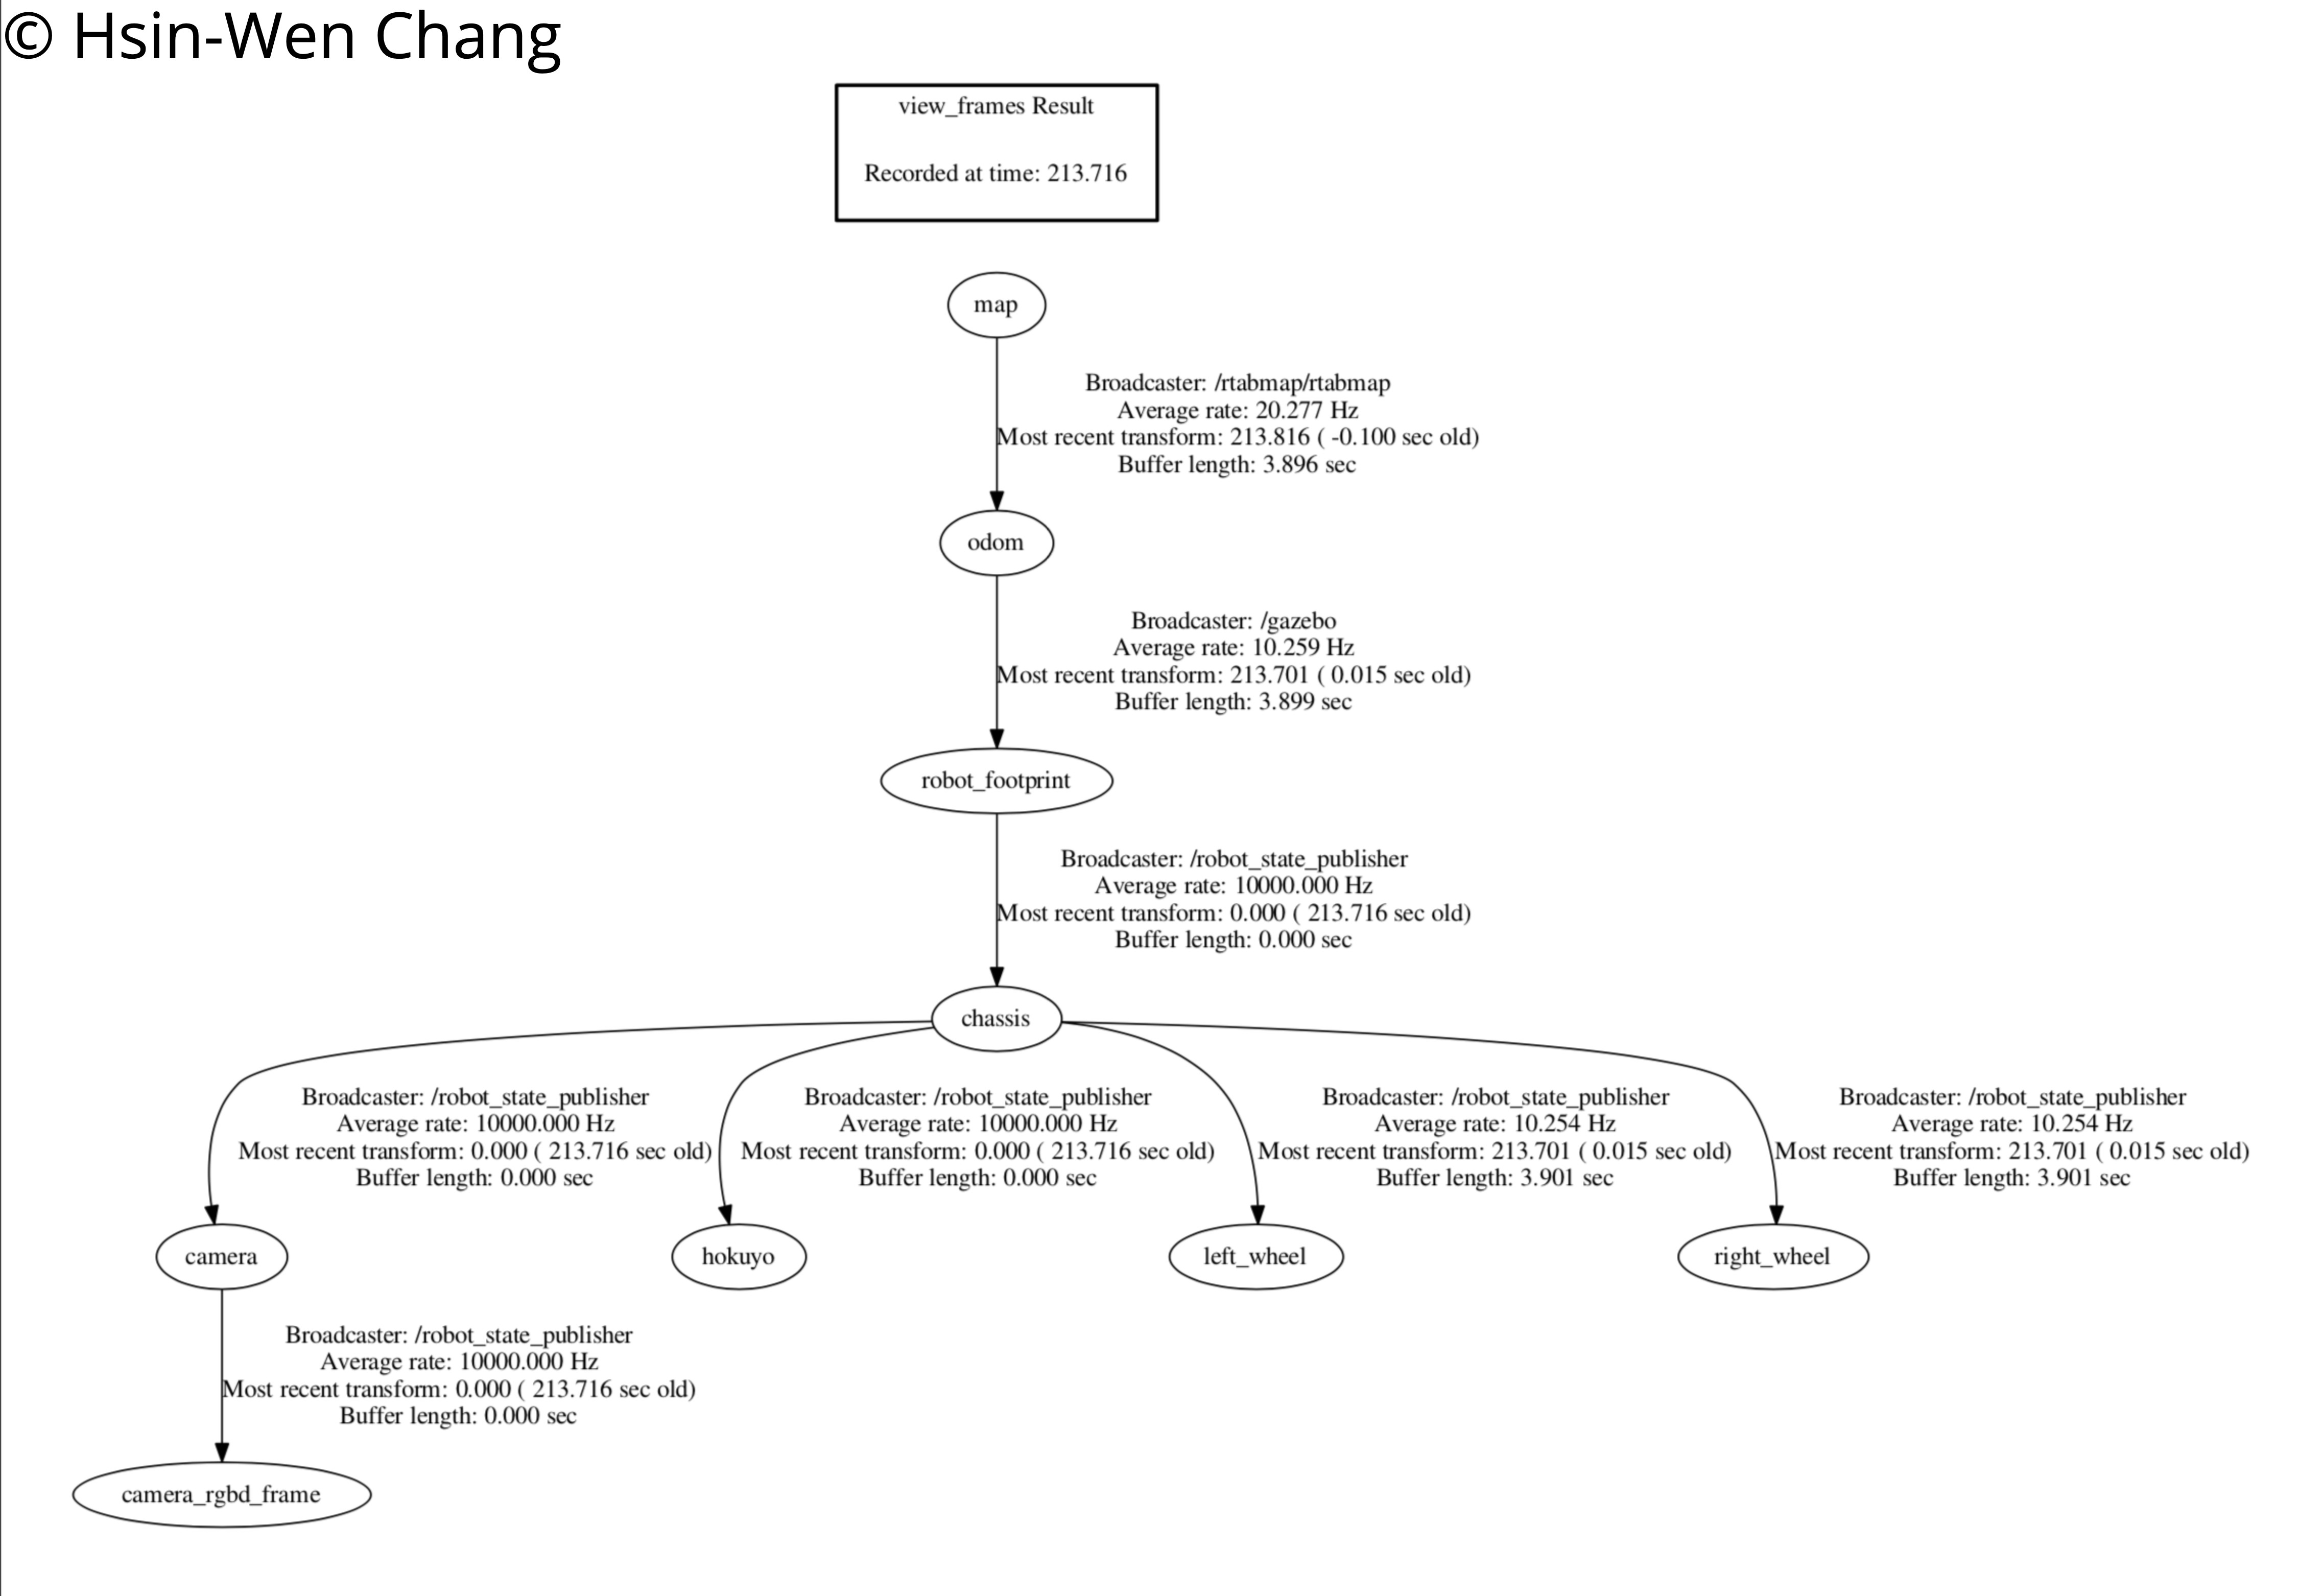
\includegraphics[width=\linewidth]{TransformFrames.png}
      \caption{Robot transformation frame.}
      \label{fig:robot1}
\end{figure}
\section{SLAM Results And Discussion}
Hsin bot was teleoped around the room and at some point failed teleop moving forward since the RTAB-MAP algorithm perform false positive loop closure. The 2D Maps of both environments are produced by laser rangefinder which mounted in front of the robot to minimize the chance to omit small obstacles in both environments. The Occupancy Grid Maps of the environments are similar to the 2D map which are base on laser scan and have the same drawbacks like 2D map. Being able to leverage RTAB-Map to visualize 3D map as point cloud from RGB-D camera, estimated trajectory and loop detection at the same time.

\begin{figure}[thpb]
      \centering
      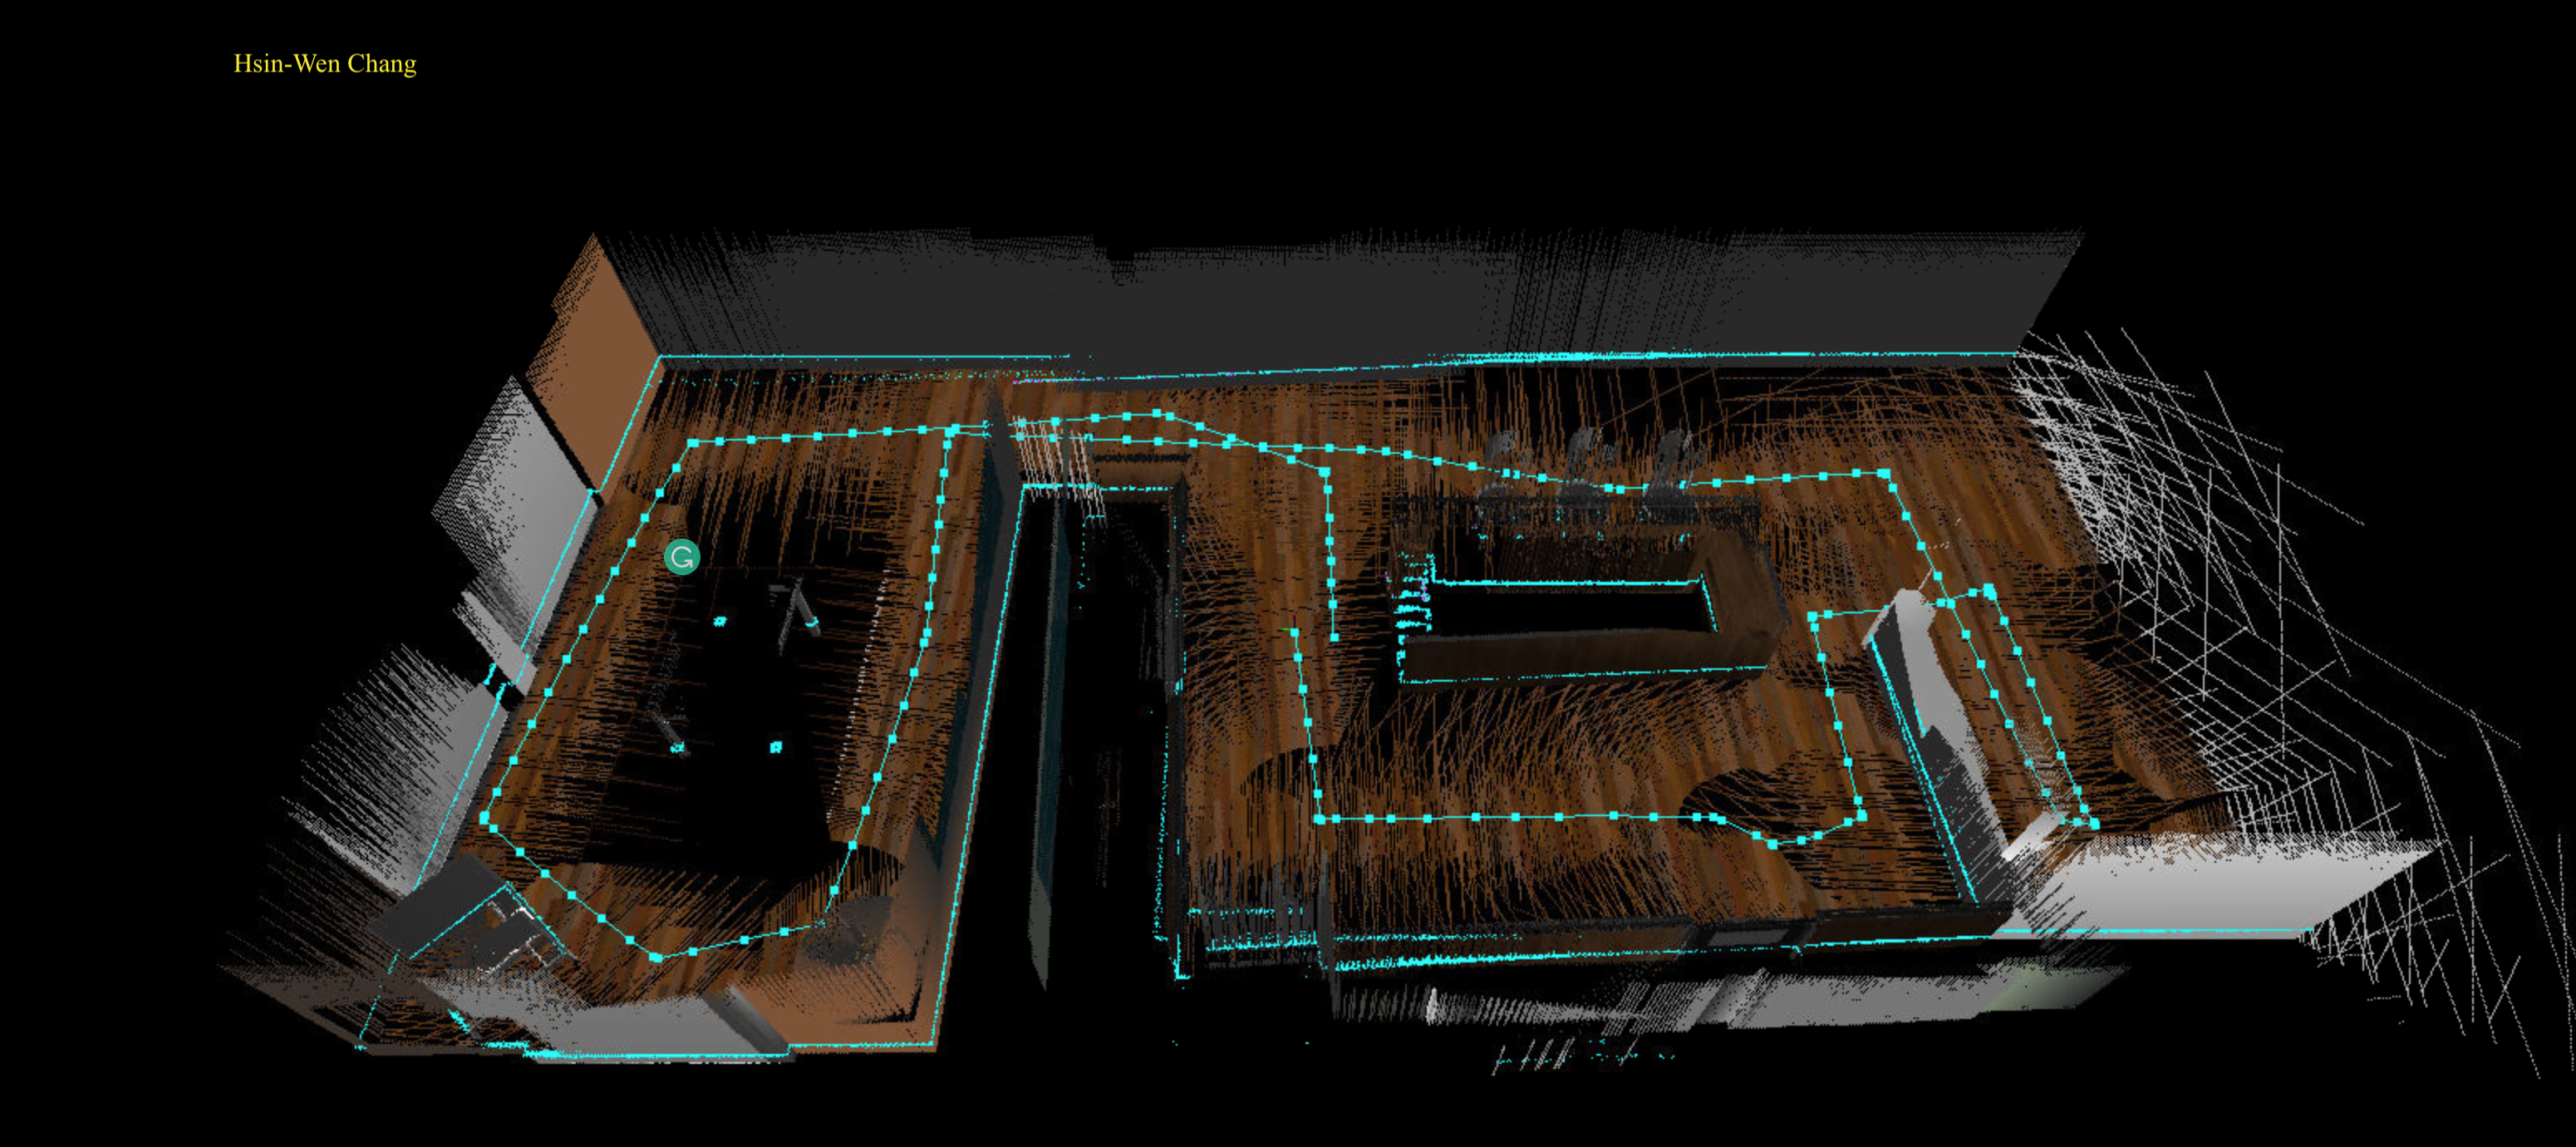
\includegraphics[width=\linewidth]{suppliedEnvironment.png}
      \caption{Kitchen and dining scene.}
      \label{fig:robot1}
\end{figure}
\begin{figure}[thpb]
      \centering
      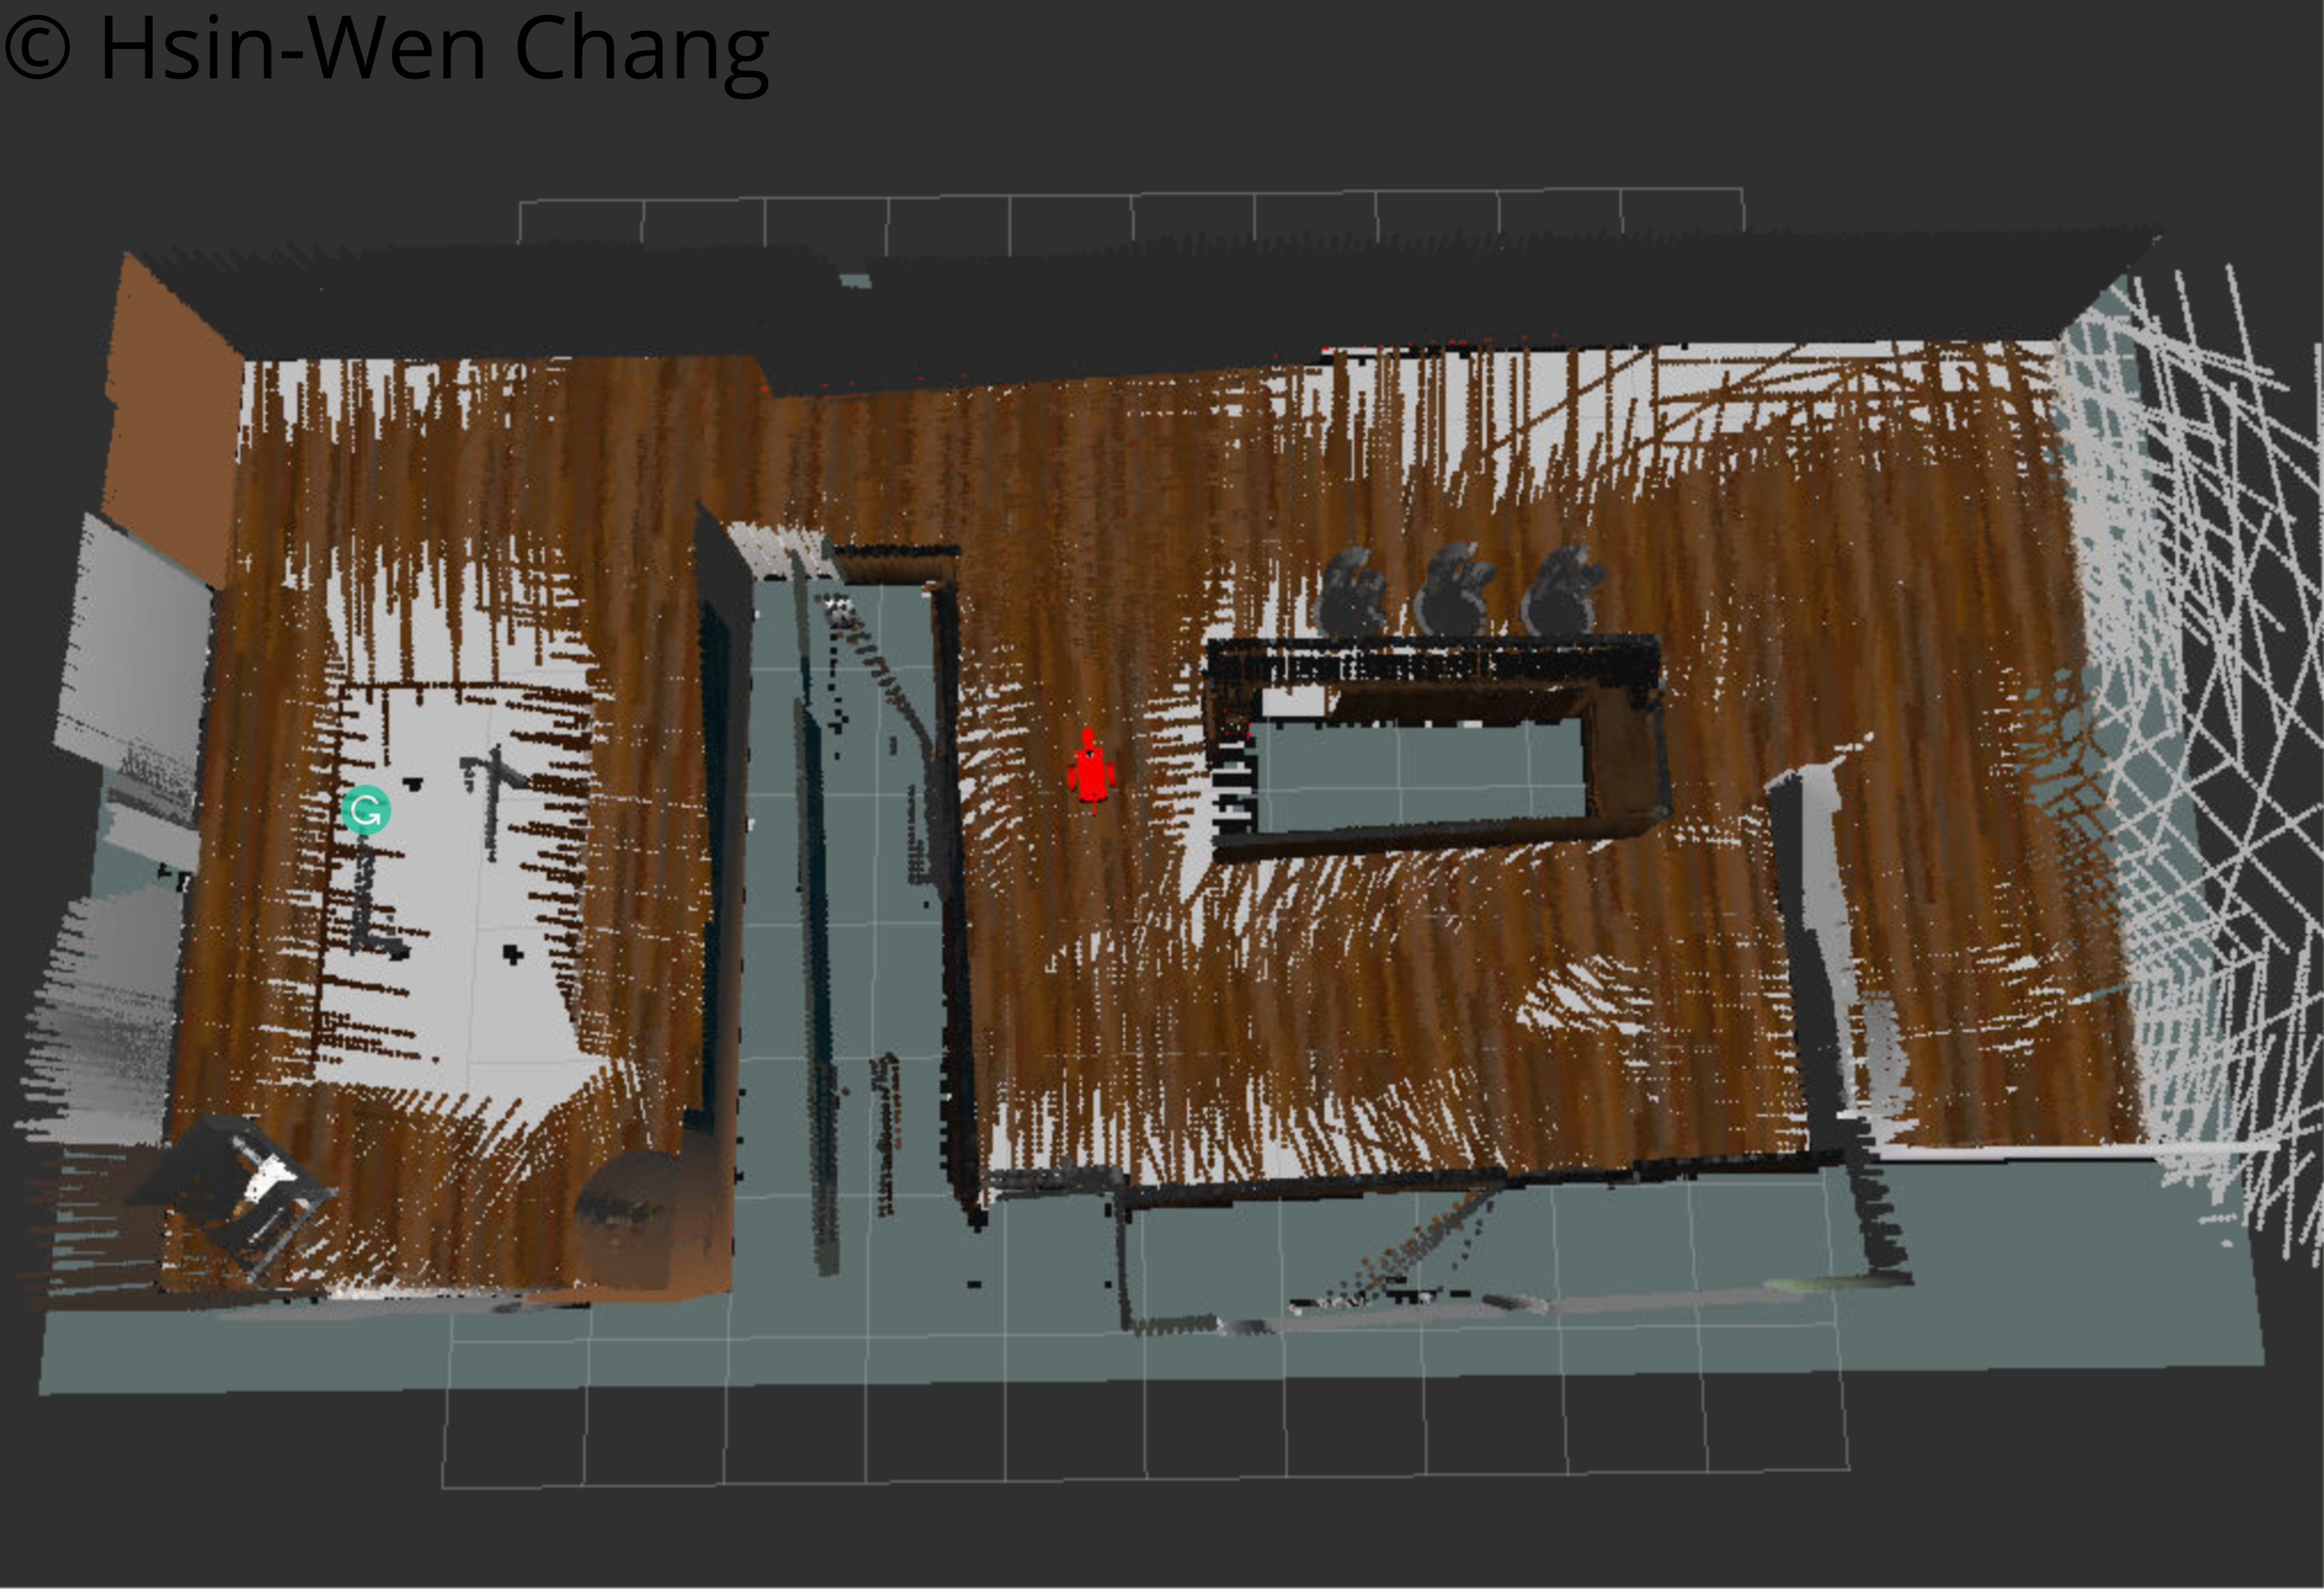
\includegraphics[width=\linewidth]{rvizMapping.png}
      \caption{Kitchen and dining scene.}
      \label{fig:robot1}
\end{figure}
\begin{figure}[thpb]
      \centering
      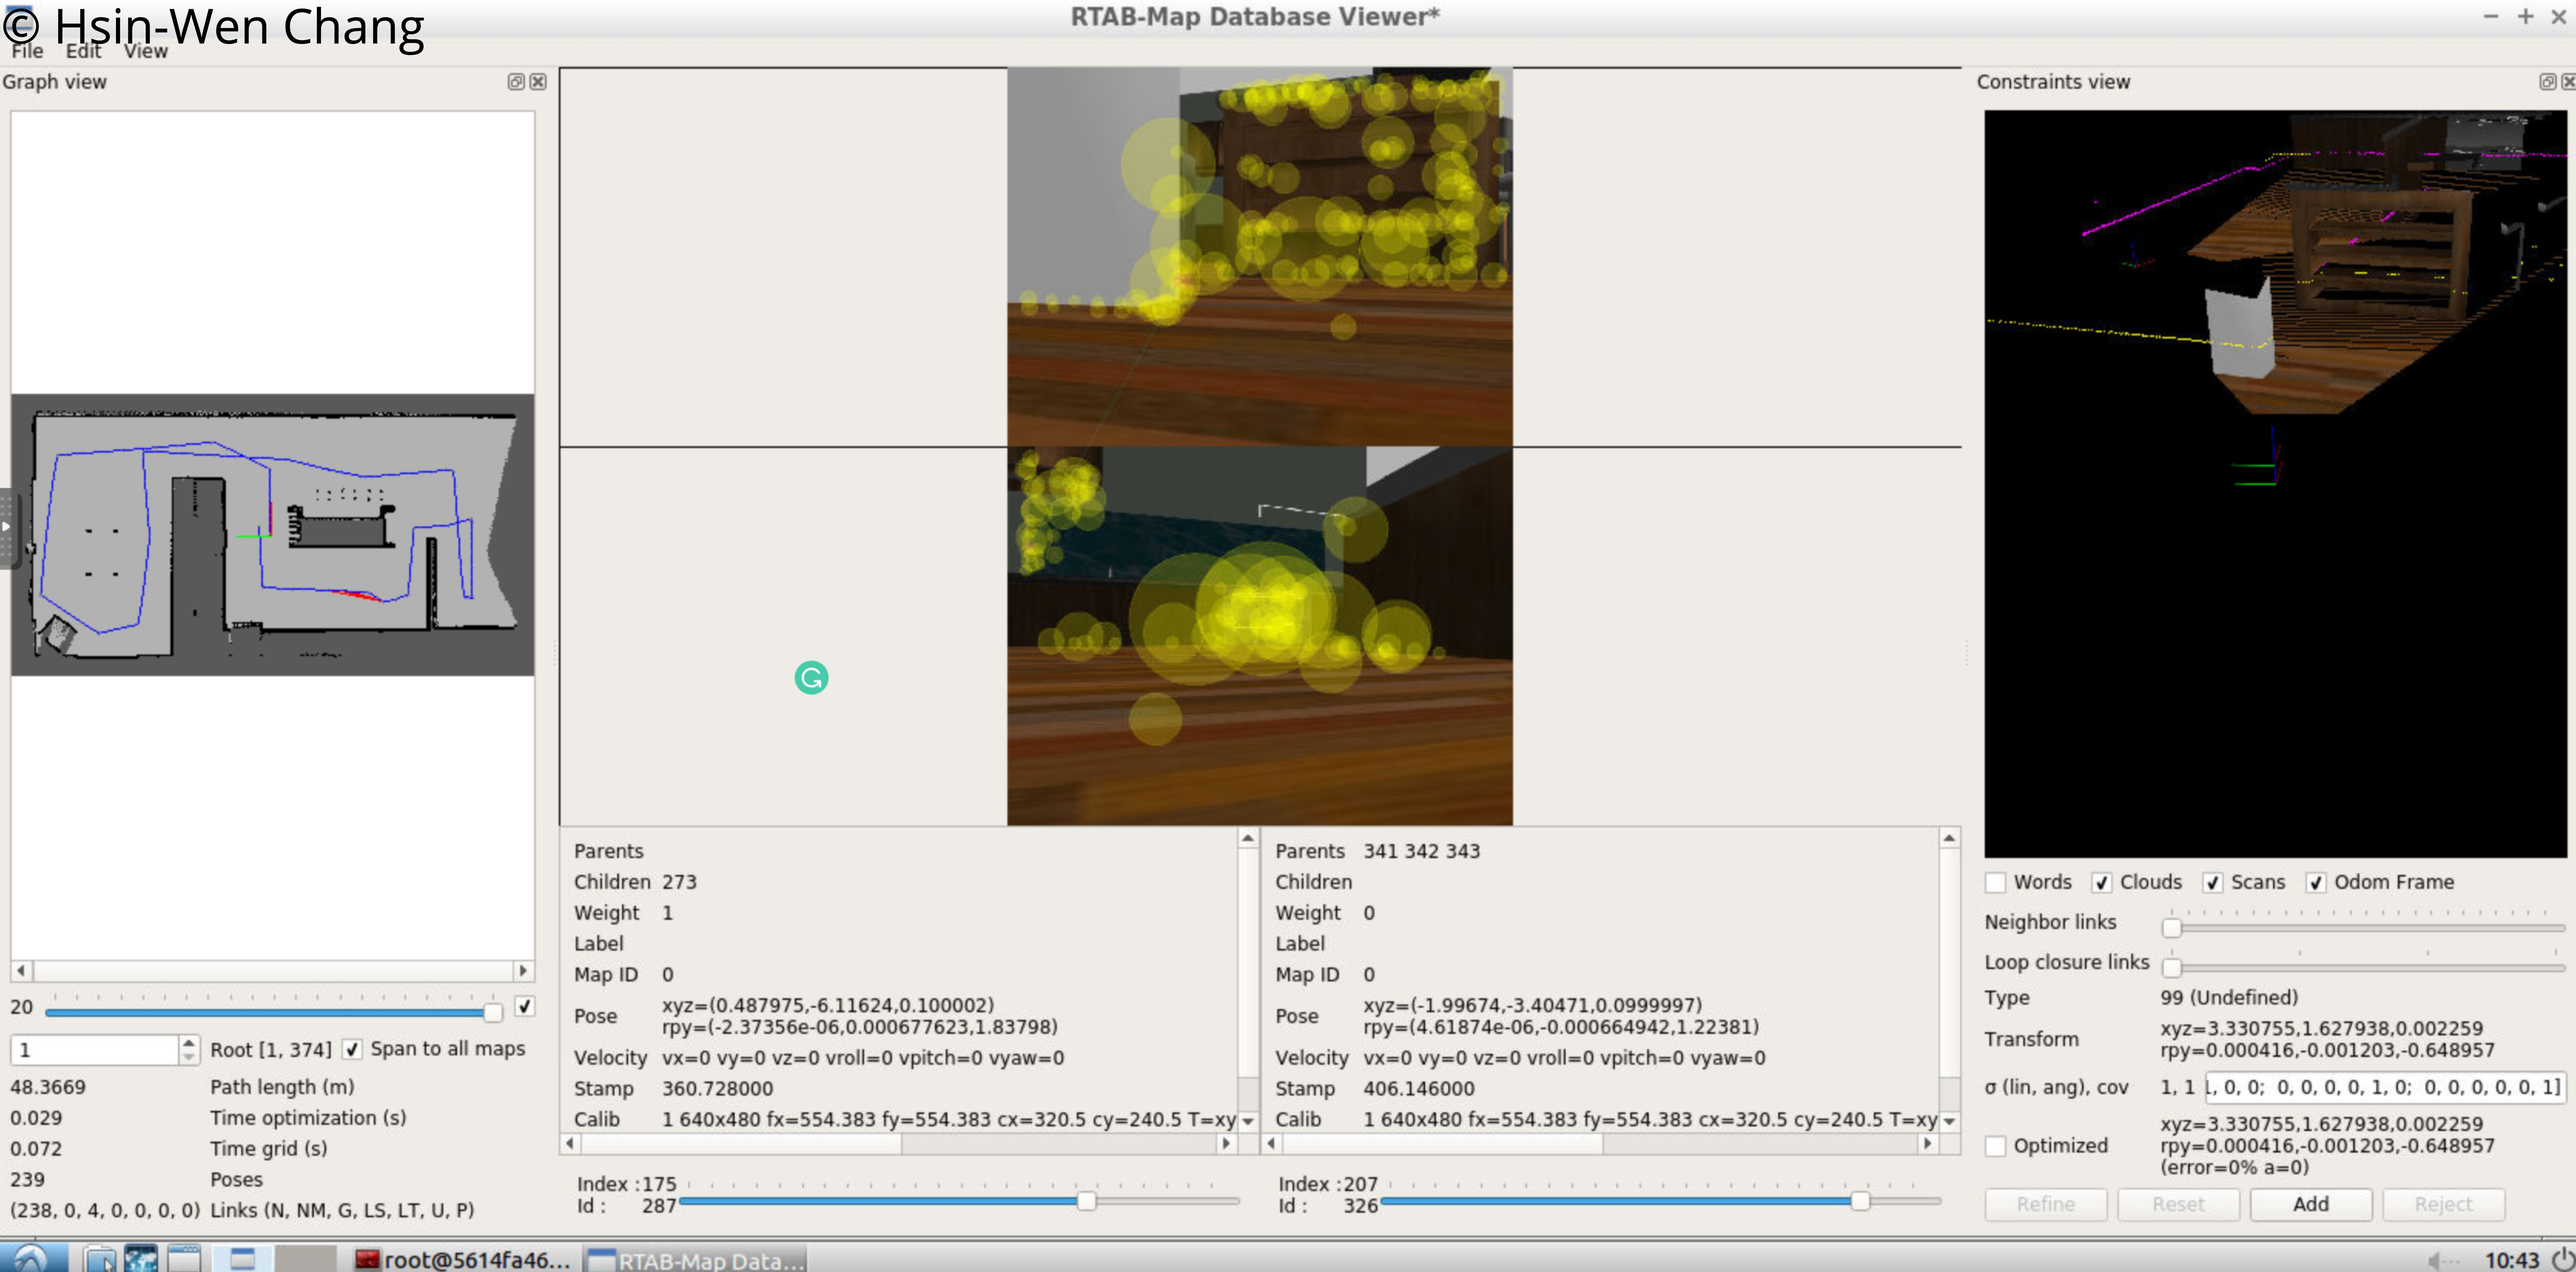
\includegraphics[width=\linewidth]{databaseViewer.png}
      \caption{Kitchen and dining scene.}
      \label{fig:robot1}
\end{figure}

\begin{figure}[thpb]
      \centering
      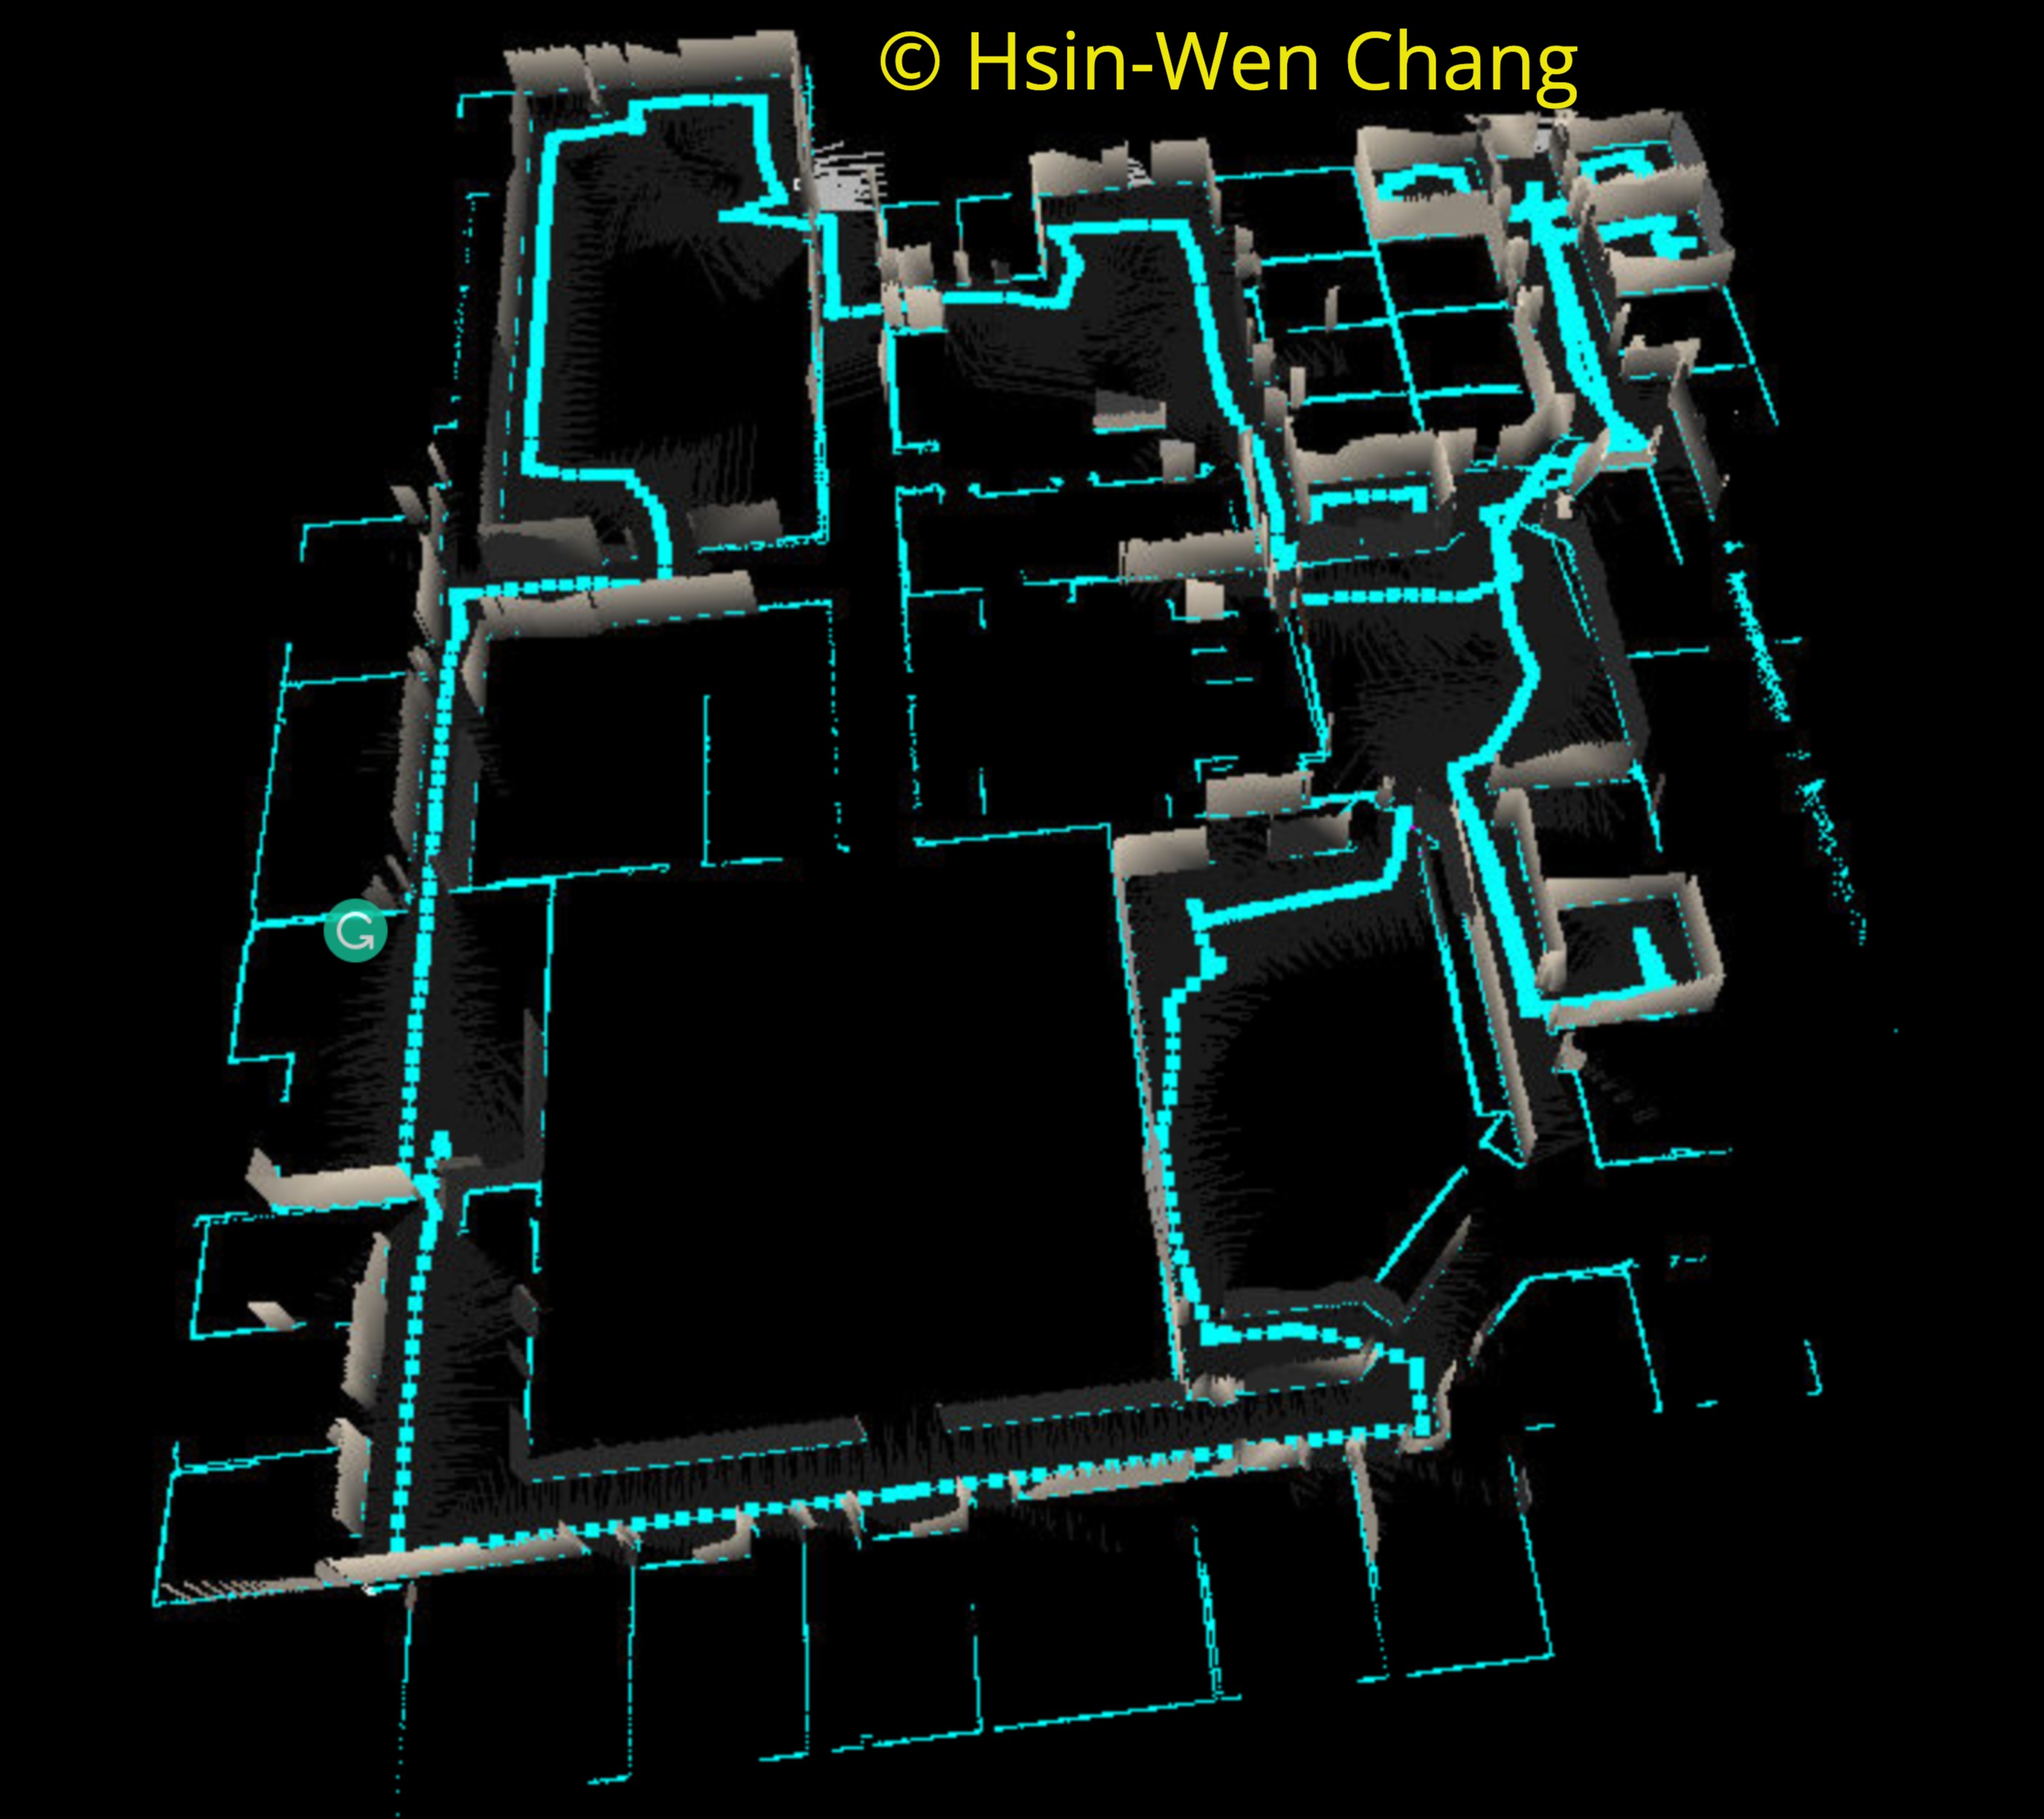
\includegraphics[width=\linewidth]{willowRTAB.png}
      \caption{Willow garage.}
      \label{fig:robot1}
\end{figure}
\begin{figure}[thpb]
      \centering
      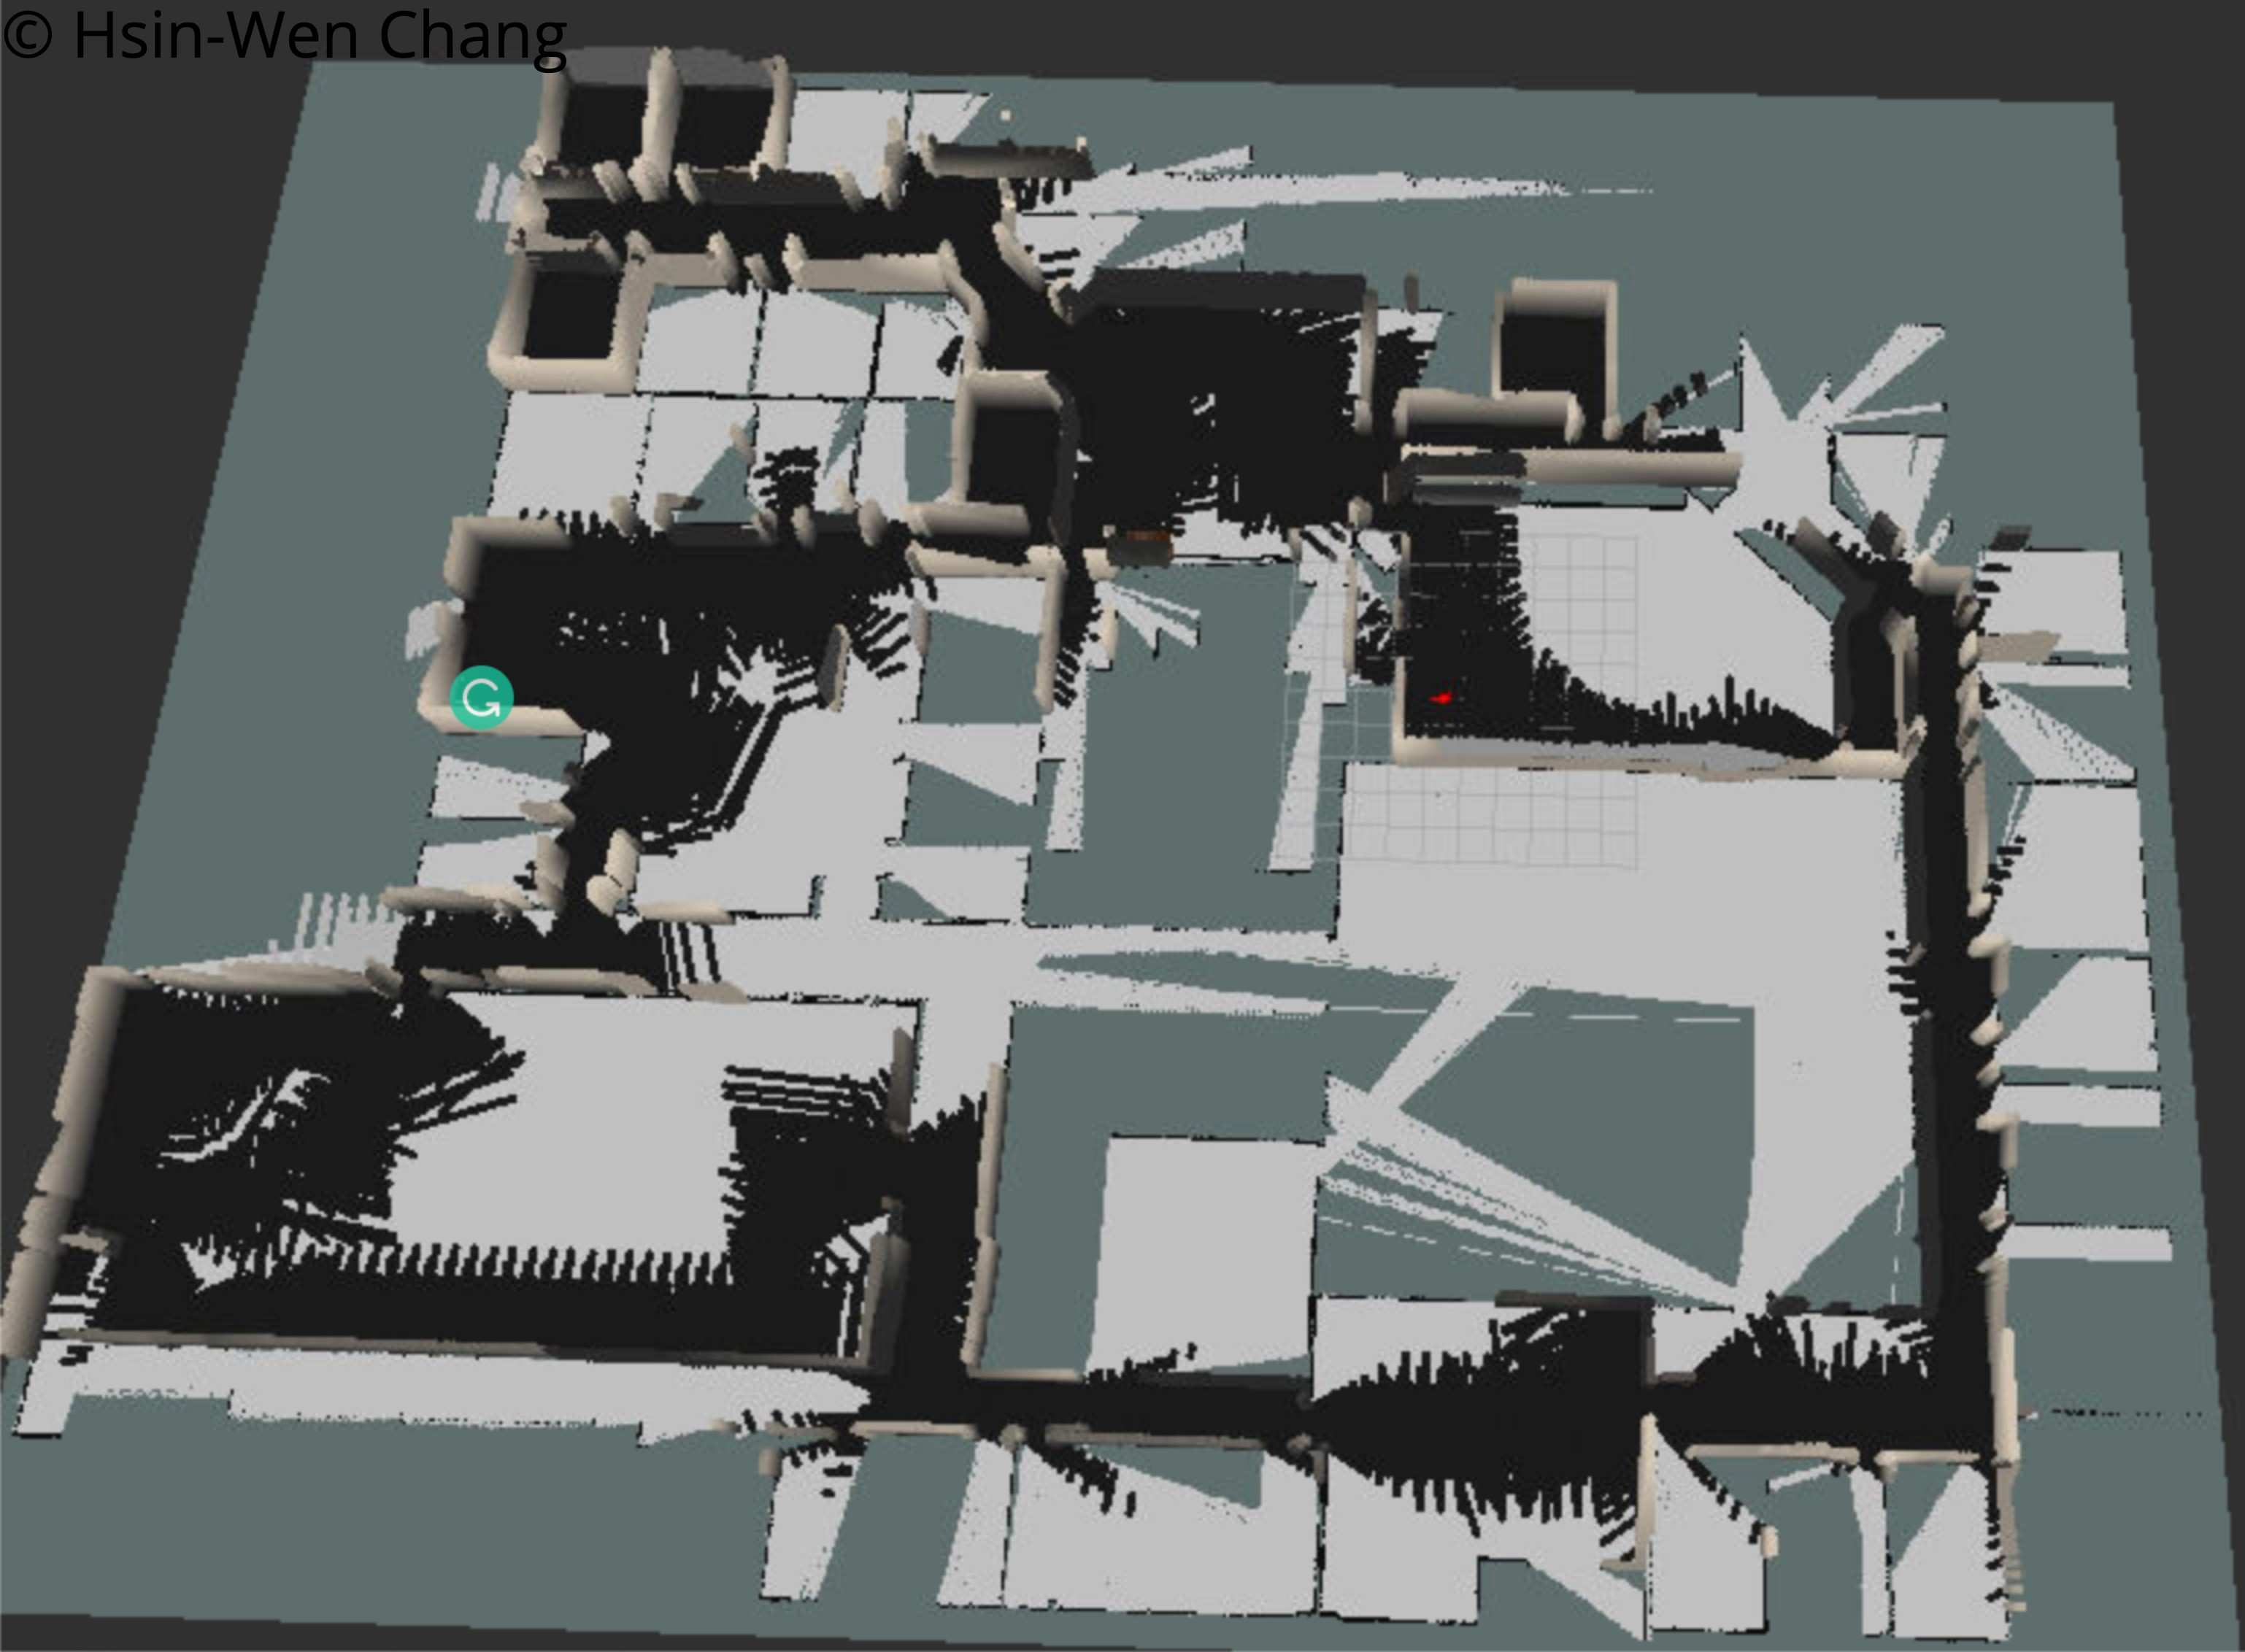
\includegraphics[width=\linewidth]{RViz.png}
      \caption{HsinBot in willow garage.}
      \label{fig:robot1}
\end{figure}
\begin{figure}[thpb]
      \centering
      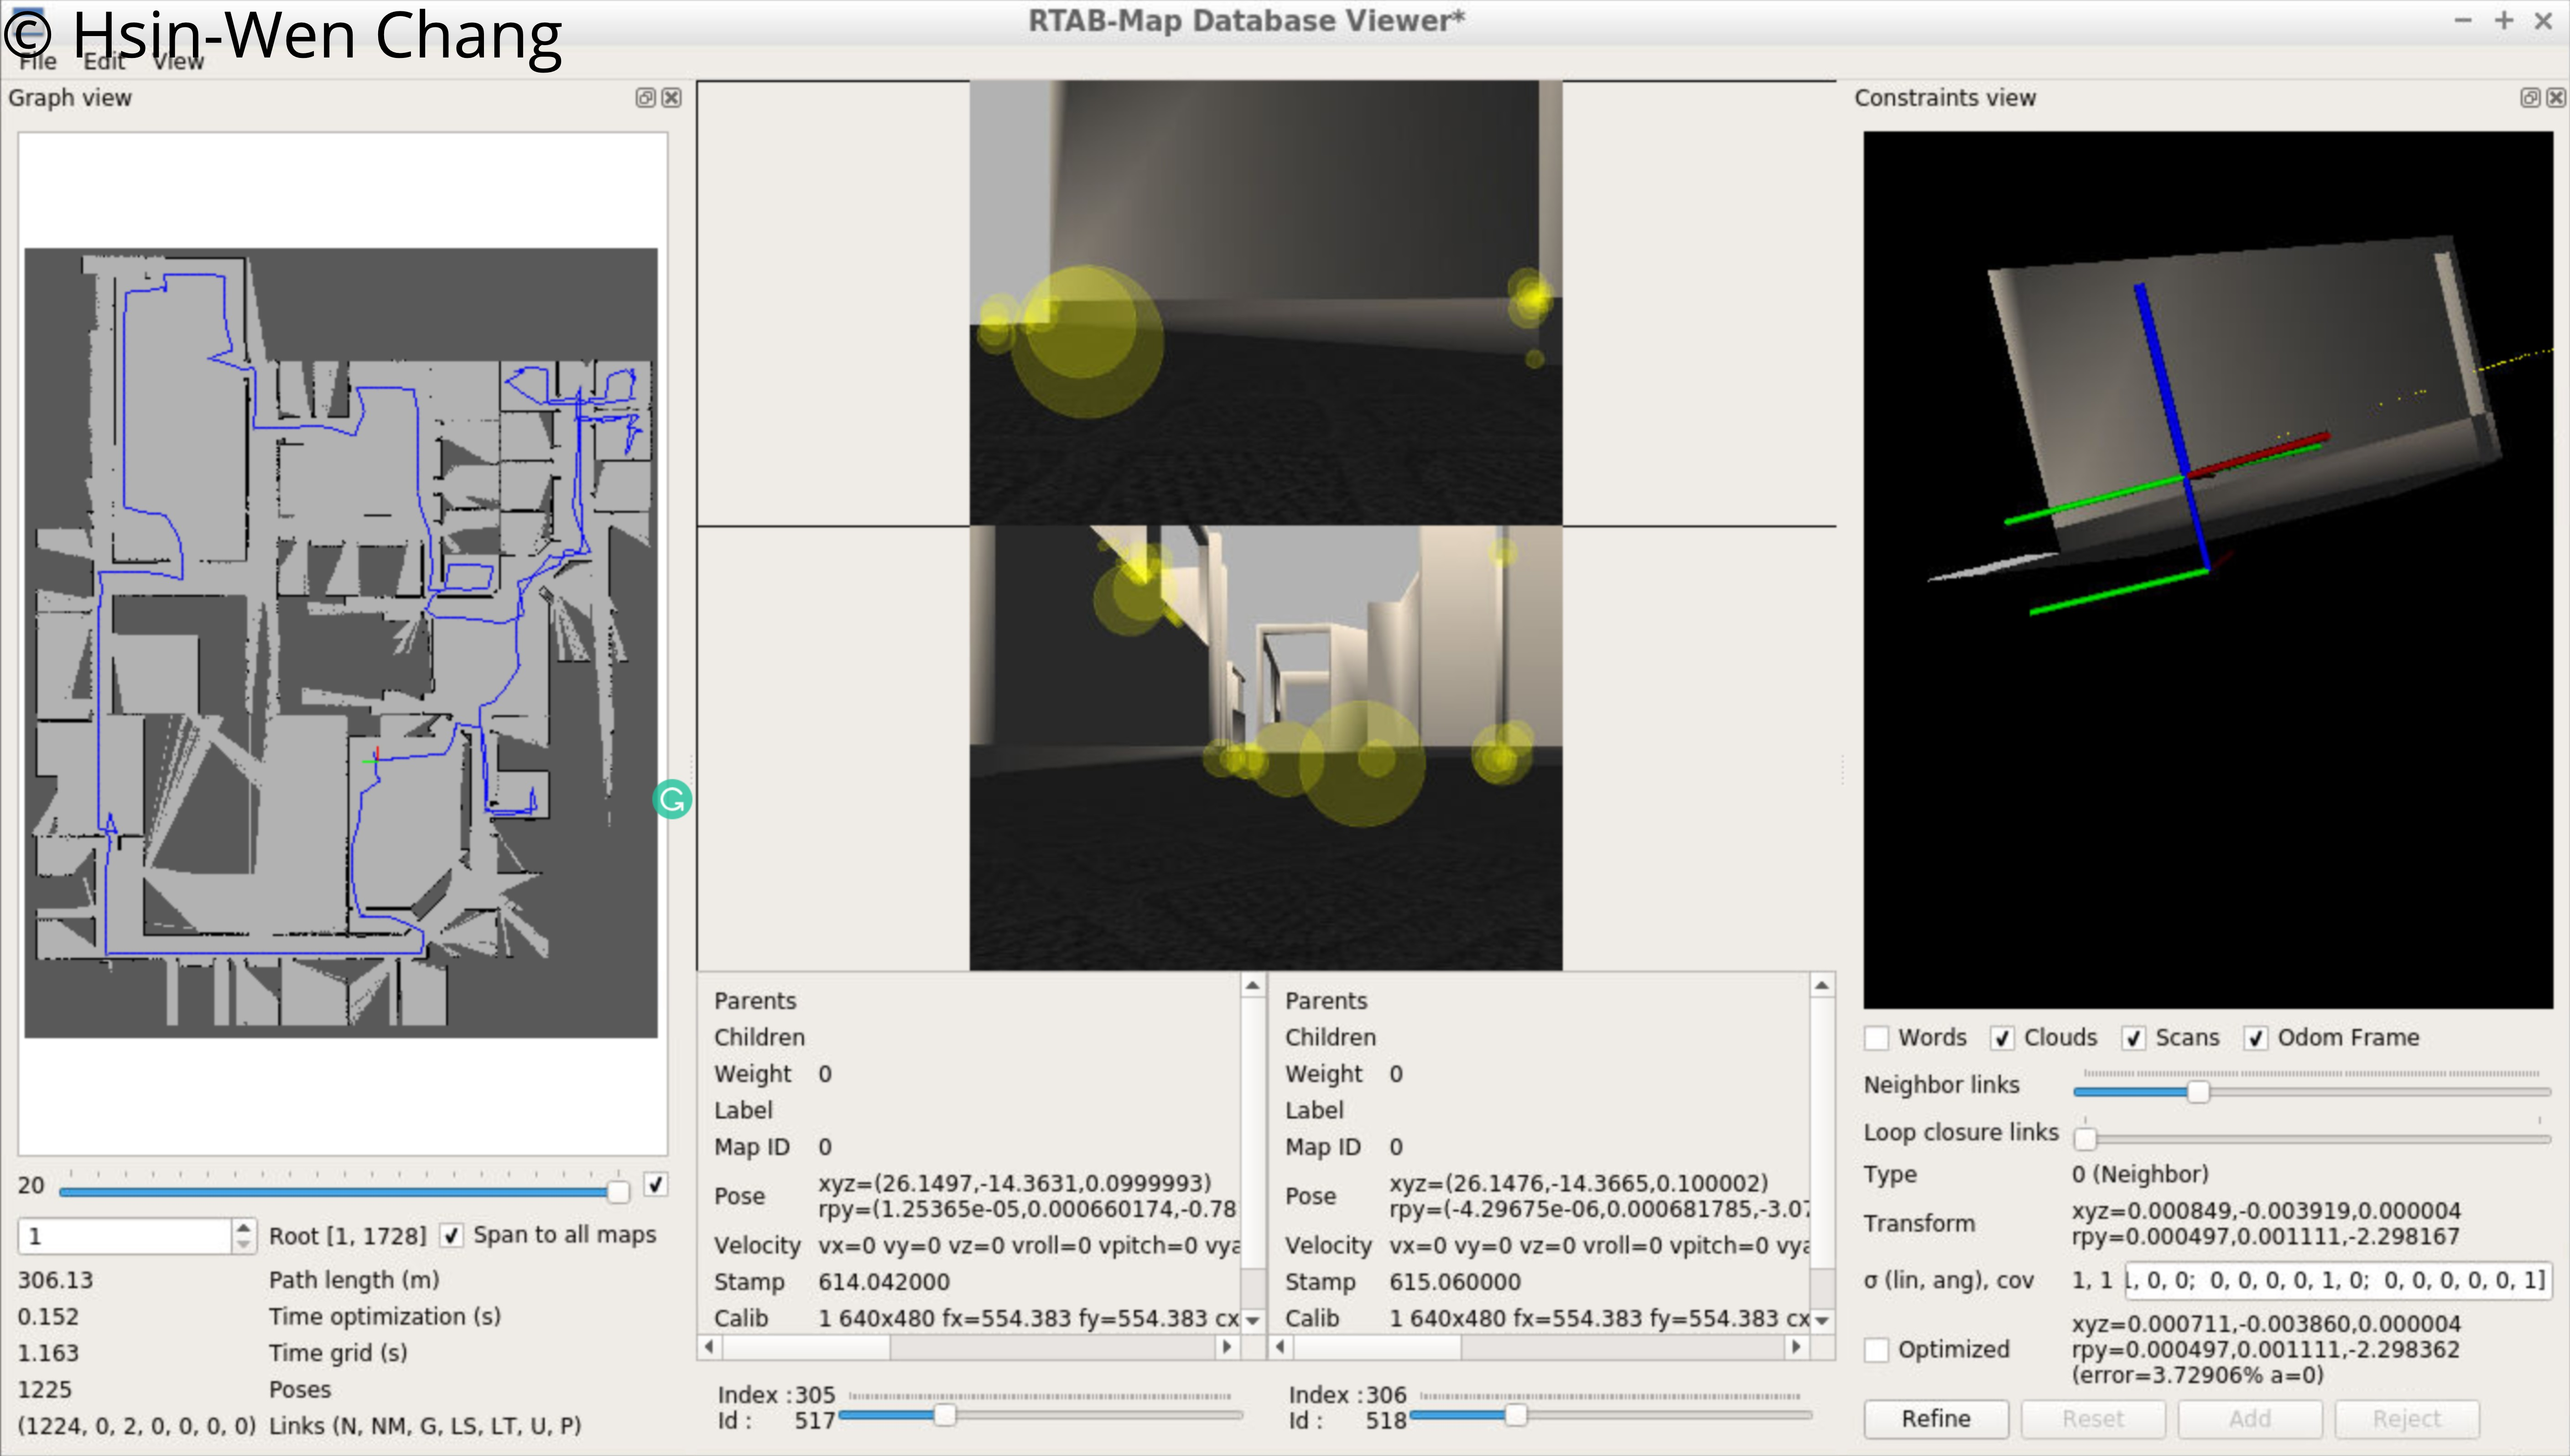
\includegraphics[width=\linewidth]{willowDBViewer.png}
      \caption{HsinBot in willow garage.}
      \label{fig:robot1}
\end{figure}

\section{Future work- Applies RTAB Mapping To A Real Robot}
 Intel Aero is using 4 ROS nodes:
\begin{itemize}
\item Communicate with the flight controller using the MAVROS node. MAVROS is designed to work with MAVLINK compatible flight controllers, like Intel Aero Flight Controller with PX4 or Arudpilot stacks.
\item Interact with the Intel Real Sense R200 camera using RealSense node.
\item As an alternative to the MAVROS node, you can access the IMU with a dedicated node imu driver. MAVROS will give you access to the entire MAVLink protocol (IMU included), imu driver will give you access to the IMU only in a simpler way. 

After launched ROS, use rossun rviz to see the RealSense output and run RTAB Mapping to see odometry is computed visually and a larger 3D model of the open space is built.
\end{itemize}
\begin{figure}[thpb]
      \centering
      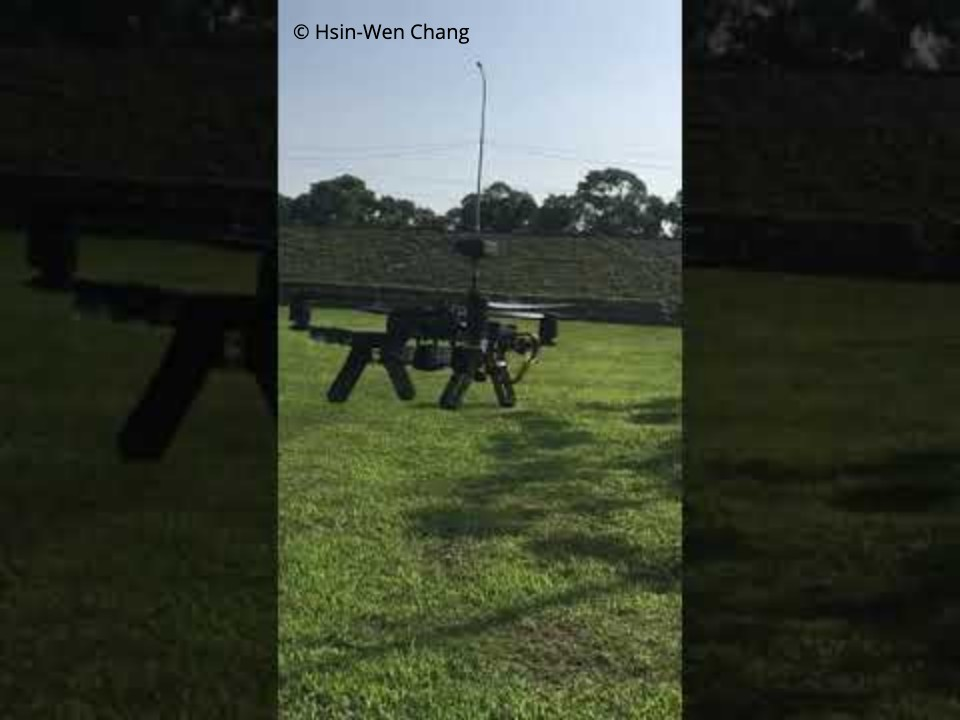
\includegraphics[width=\linewidth]{aero.jpeg}
      \caption{Intel aero Flying Car.}
      \label{fig:robot1}
\end{figure}
\begin{figure}[thpb]
      \centering
      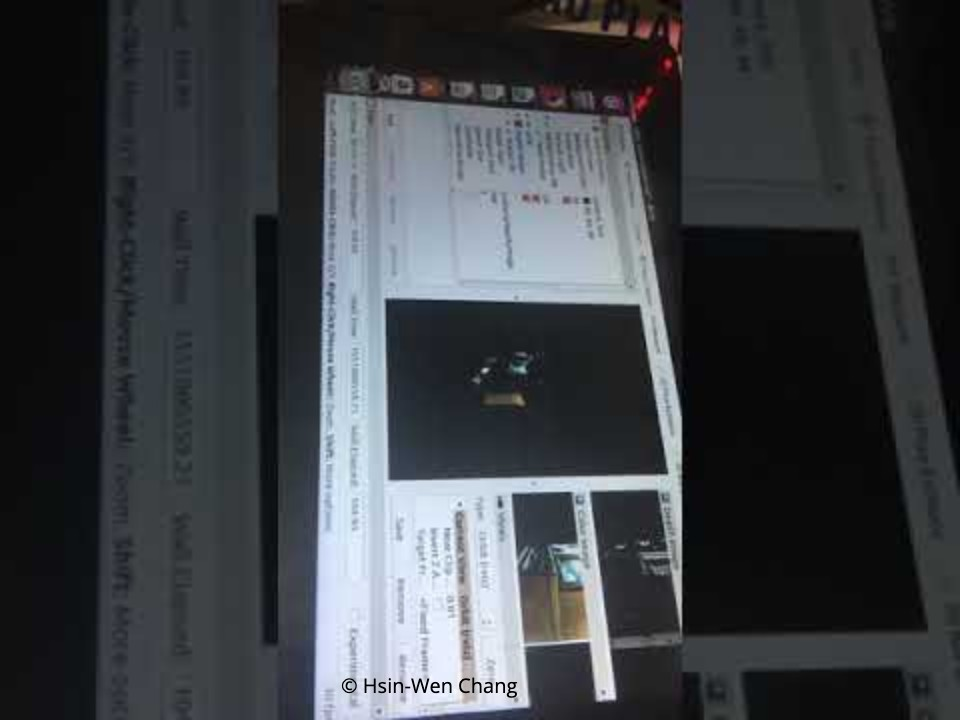
\includegraphics[width=\linewidth]{RTAB-Map.jpeg}
      \caption{Deploys RTAB-Map on the Intel aero Flying Car.}
      \label{fig:robot1}
\end{figure}

\bibliography{bib}
\bibliographystyle{ieeetr}
[1] The GraphSLAM Algorithm with Applications to Large-Scale Mapping of Urban Structures, Sebastian Thrun, Michael Montemerlo
, Stanford AI Lab,Stanford University {thrun,mmde}@stanford.edu. THE INTERNATIONAL JOURNAL OF ROBOTICS RESEARCH / May–June 2006
\end{document}
